\documentclass[12pt]{report}

\usepackage[utf8]{inputenc}
\usepackage[spanish, english]{babel}
\usepackage{graphicx}
\usepackage{amssymb, amsmath, amsthm}
\usepackage{bm} % For boldface greek letters
\usepackage{hyperref} % Para poder tener hyperlinks
\usepackage{enumerate}
\usepackage{calligra} % Para dedicacion
\usepackage[sorting=none]{biblatex} \addbibresource{bibliografia.bib}
\usepackage{csquotes}

\usepackage[normalem]{ulem} % For strikethrough with command \sout
\usepackage{slashed} % For slashed in Dirac operator

%%%%%% Mis Codigos

% TODO notes package
\usepackage{xargs}                  % Use more than one optional parameter in a new command
\usepackage[pdftex,dvipsnames]{xcolor}
%\usepackage{xargs}                      % Use more than one optional parameter in a new
%\usepackage[pdftex,dvipsnames]{xcolor}  % Coloured text etc.

%
%\usepackage[colorinlistoftodos,prependcaption,textsize=tiny]{todonotes}
\usepackage[disable]{todonotes}

\newcommandx{\unsure}[2][1=]{\todo[linecolor=red,backgroundcolor=red!25,bordercolor=red,#1]{#2}}
\newcommandx{\change}[2][1=]{\todo[linecolor=blue,backgroundcolor=blue!25,bordercolor=blue,#1]{#2}}
\newcommandx{\complete}[2][1=]{\todo[linecolor=pink,backgroundcolor=pink!25,bordercolor=blue,#1]{#2}}
\newcommandx{\info}[2][1=]{\todo[linecolor=OliveGreen,backgroundcolor=OliveGreen!25,bordercolor=OliveGreen,#1]{#2}}
\newcommandx{\improvement}[2][1=]{\todo[linecolor=Plum,backgroundcolor=Plum!25,bordercolor=Plum,#1]{#2}}
\newcommandx{\thiswillnotshow}[2][1=]{\todo[disable,#1]{#2}}

% Colored text and boxes with my color conventions for highlighting
\usepackage[dvipsnames]{xcolor}
%\usepackage[dvipsnames]{xcolor}

%
% \newcommand{\ytext}[1]{\textcolor{yellow}{#1}}
% \newcommand{\otext}[1]{\textcolor{orange}{#1}}
% \newcommand{\rtext}[1]{\textcolor{red}{#1}}
% \newcommand{\lbtext}[1]{\textcolor{cyan}{#1}}
% \newcommand{\dbtext}[1]{\textcolor{blue}{#1}}
% \newcommand{\ptext}[1]{\textcolor{Plum}{#1}}
% \newcommand{\lgtext}[1]{\textcolor{LimeGreen}{#1}}
% \newcommand{\dgtext}[1]{\textcolor{OliveGreen}{#1}}

\newcommand{\ytext}[1]{\textcolor{black}{#1}}
\newcommand{\otext}[1]{\textcolor{black}{#1}}
\newcommand{\rtext}[1]{\textit{#1}}
\newcommand{\lbtext}[1]{\textcolor{black}{#1}}
\newcommand{\dbtext}[1]{\textcolor{black}{#1}}
\newcommand{\ptext}[1]{\textcolor{black}{#1}}
\newcommand{\lgtext}[1]{\textcolor{black}{#1}}
\newcommand{\dgtext}[1]{\textcolor{black}{#1}}



\newcommand{\ybox}[1]{\colorbox{yellow}{#1}}
\newcommand{\obox}[1]{\colorbox{orange}{#1}}
\newcommand{\rbox}[1]{\colorbox{Salmon}{#1}}
\newcommand{\lbbox}[1]{\colorbox{SkyBlue}{#1}}
\newcommand{\dbbox}[1]{\colorbox{NavyBlue}{#1}}
\newcommand{\pbox}[1]{\colorbox{Plum}{#1}}
\newcommand{\lgbox}[1]{\colorbox{LimeGreen}{#1}}
\newcommand{\dgbox}[1]{\colorbox{OliveGreen}{#1}}



% Math symbols
\usepackage{xparse}

%\usepackage{amssymb,amsmath,amsthm}
%\usepackage{xparse}

%%% Common symbols redifined
\let\oldepsilon\epsilon
\renewcommand{\epsilon}{\varepsilon}
\renewcommand{\varepsilon}{\oldepsilon}

\let\oldphi\phi
\renewcommand{\phi}{\varphi}
\renewcommand{\varphi}{\oldphi}

\newcommand{\emty}{\varnothing}
\newcommand{\varempty}{\nothing}

%%% Common Sets
\newcommand{\bb}[1]{\ensuremath{\mathbb{#1}} }
\newcommand{\ZZ}{\ensuremath{\mathbb{Z}} }
\newcommand{\NN}{\ensuremath{\mathbb{N}} }
\newcommand{\QQ}{\ensuremath{\mathbb{Q}} }
\newcommand{\RR}{\ensuremath{\mathbb{R}} }
\newcommand{\CC}{\ensuremath{\mathbb{C}} }


\newcommand{\iss}{\cong}  % Isomorphism symbol, here it is the one with a tilde

%%%%%%%%%%%%%% Sets

\newcommand{\set}[1]{\ensuremath{\left\{ #1 \right\}}} % Set function, simply puts nice left and right braces
\newcommand{\st}{\ensuremath{\ |\ }} % Such that symbol, TODO improve

\newcommand{\psubset}{\ensuremath{\subset}}
\renewcommand{\subset}{\ensuremath{\subseteq}} % Subset symbol, in this case it is the subset or equal to symbol

\newcommand{\bunion}{\bigcup}
%\newcommand{\biun}{\bun^{\infty}}
%\newcommand{\bfun}[3][n]{\bun_{#1 = #2}^{#3}}
\newcommand{\union}{\cup}
%\newcommand{\siun}{\sun^{\infty}}
%\newcommand{\sfun}[3][n]{\sun_{#1 = #2}^{#3}}

\newcommand{\binter}{\bigcap}
%\newcommand{\biinter}{\binter^{\infty}}
%\newcommand{\bfifter}[3][n]{\binter_{#1 = #2}^{#3}}
\newcommand{\inter}{\cap}
%\newcommand{\sininter}{\sinter^{\infty}}
%\newcommand{\sfinter}[3][n]{\sinter_{#1 = #2}^{#3}}

%%%%%% Calculus

% Integrals

%% Single Integrals
\NewDocumentCommand \integ {s O{} O{} m o}
{
	\IfBooleanTF{#1}{\oint}{\int}_{#2}^{#3} #4 %
	\IfNoValueF {#5} {\mathrm{d} #5}
}

%% Derivatives

% Normal derivative
% Example: \der[n]{f}{x}[x_0]
\NewDocumentCommand \der {O{} m m o}
{
	\frac{\mathrm{d}^{#1} #2}{\mathrm{d} {#3}^{#1}}%
	\IfNoValueF{#4} {\biggr|_{#4}}
}

%% Partial Derivatives

% With respect to one variable
% Example: \pder[n]{f}{y}[\pthvars[x_0][y_0][z_0]][(x, z)
\NewDocumentCommand \pder {O{} m m O{} o}
{
    \ensuremath{
	\IfNoValueTF {#5}
	{
		\frac{\partial^{#1} #2}{\partial {#3}^{#1}} #4
	}
	{
		\left(%
		\frac{\partial^{#1} #2}{\partial {#3}^{#1}}%
		\right)_{#5}  #4
	}
	}
}

% With respecto to two variables
% Example: \twpder{g}{y}{x}[(x_0, y_0)]
\NewDocumentCommand \twpder {m m m O{}}
{
	\frac{\partial^2 #1}{\partial #2 \partial #3} #4
}

\newcommand{\abs}[1]{\left\lvert #1 \right\rvert}
\newcommand{\norm}[1]{\left\lVert #1 \right\rVert}

% Physics symbols (vectors, units)
\usepackage{tikz}
% Version of December 26 2016

%%%%%%%%%%%%%%%%%%%%%%%%%%%%%%%%%%%%%%%%%%% Vectors

%%%%%%%% For SI units %%%%%%%
%\usepackage{siunitx}

%%%%%%%% Vectors %%%%%%%%%%%% (Just see last lines)
%\usepackage{tikz}         % For arrow and dots in \xvec

% --- Macro \xvec
\makeatletter
\newlength\xvec@height%
\newlength\xvec@depth%
\newlength\xvec@width%
\newcommand{\xvec}[2][]{%
  \ifmmode%
    \settoheight{\xvec@height}{$#2$}%
    \settodepth{\xvec@depth}{$#2$}%
    \settowidth{\xvec@width}{$#2$}%
  \else%
    \settoheight{\xvec@height}{#2}%
    \settodepth{\xvec@depth}{#2}%
    \settowidth{\xvec@width}{#2}%
  \fi%
  \def\xvec@arg{#1}%
  \def\xvec@dd{:}%
  \def\xvec@d{.}%
  \raisebox{.2ex}{\raisebox{\xvec@height}{\rlap{%
    \kern.05em%  (Because left edge of drawing is at .05em)
    \begin{tikzpicture}[scale=1]
    \pgfsetroundcap
    \draw (.05em,0)--(\xvec@width-.05em,0);
    \draw (\xvec@width-.05em,0)--(\xvec@width-.15em, .075em);
    \draw (\xvec@width-.05em,0)--(\xvec@width-.15em,-.075em);
    \ifx\xvec@arg\xvec@d%
      \fill(\xvec@width*.45,.5ex) circle (.5pt);%
    \else\ifx\xvec@arg\xvec@dd%
      \fill(\xvec@width*.30,.5ex) circle (.5pt);%
      \fill(\xvec@width*.65,.5ex) circle (.5pt);%
    \fi\fi%
    \end{tikzpicture}%
  }}}%
  #2%
}
\makeatother

% --- Override \vec with an invocation of \xvec.
\let\stdvec\vec
\renewcommand{\vec}[1]{\xvec[]{#1}}                             % Vector
% --- Define \dvec and \ddvec for dotted and double-dotted vectors.
\newcommand{\tvec}[1]{\xvec[.]{#1}}                             % Vector derived wrt time
\newcommand{\ttvec}[1]{\xvec[:]{#1}}                            % Vector derived twice wrt time


% Theorem environments
% %Version of October 8, 2016

%\usepackage{amsthm}

\theoremstyle{definition} %To avoid the annoying italics all the time, and to not sloppily redefine all of them 

\newtheorem{theo}{Theorem}[section]  %numbered according to section environment, so in section to it restarts as 2.1 
\newtheorem{prop}{Proposition}[section]  %numbered according to section environment, so in section to it restarts as 2.1 
\newtheorem{lemma}[theo]{Lemma}     %numbering shared with theorem 
\newtheorem{defn}{Definition}[section]   
\newtheorem{coro}{Corollary}[theo]


\theoremstyle{remark} 
\newtheorem*{remark}{Remark} 
 
%\let\oldtheo\theo 
%\renewcommand{\theo}{\oldtheo\normalfont}  
%  
%\let\olddefn\defn  
%\renewcommand{\defn}{\olddefn\normalfont}  
%  
%\let\oldlemma\lemma  
%\renewcommand{\lemma}{\oldlemma\normalfont}  
%  
%\let\oldcoro\coro  
%\renewcommand{\coro}{\oldcoro\normalfont}

%%%%%%%% ``Example'' environment, very basic, doesnt work with itemize
\theoremstyle{definition}

\newtheorem*{exmp}{Example}

\usepackage{tikz-cd} %To do Commutative Diagrams

% Extras
\newcommand{\linea}{\rule{10cm}{1mm}}
\usepackage{ulem}
\renewcommand{\theequation}{\thechapter.\arabic{equation}} % To label Ch 0 equations as 0.1, 0.2, etc

%%%%%%%
\newenvironment{dedication}
  {\clearpage           % we want a new page
   \thispagestyle{empty}% no header and footer
   \vspace*{\stretch{1}}% some space at the top 
   \raggedleft          % flush to the right margin
  }
  {\par % end the paragraph
   \vspace{\stretch{3}} % space at bottom is three times that at the top
   \clearpage           % finish off the page
  }

%%%%%%%
\graphicspath{ {images/} }

%%%%%%%
\theoremstyle{definition}
\newtheorem{example}{Example}[section]
\newtheorem{definition}[example]{Definition}
\newtheorem{theorem}[example]{Theorem}
\newtheorem{proposition}[example]{Proposition}
\newtheorem{lemma}[example]{Lemma}
\newtheorem{corollary}[example]{Corollary}
\newtheorem{notation}[example]{Notation}
\newtheorem{remark}[example]{Remark}

\usepackage{environ}

\NewEnviron{eqnsplit}{%
  \begin{equation}
  \begin{split}
    \BODY
  \end{split}
  \end{equation}
}

\NewEnviron{eqnsplit*}{%
  \begin{equation*}
  \begin{split}
    \BODY
  \end{split}
  \end{equation*}
}

% Compile document without proofs
\usepackage{comment}

%\excludecomment{proof}
%%%%%%%

% \DeclareMathOperator{\HH}{\bb H}
% \DeclareMathOperator{\FF}{\bb F}
% \DeclareMathOperator{\diffeo}{\cong}
% \DeclareMathOperator{\tr}{tr}

% \DeclareMathOperator{\Diff}{\textit{Diff}}
% \DeclareMathOperator{\Hom}{\textit{Hom}}
% \DeclareMathOperator{\End}{\textit{End}}
% \DeclareMathOperator{\Alt}{\textit{Alt}}
% \DeclareMathOperator{\Sym}{\textit{Sym}}


% \newcommand{\algeb}[1]{\mathfrak{#1}}
% \newcommand{\alg}[1]{\mathfrak{#1}}
% \newcommand{\oid}[1]{\ensuremath{\mathfrak{#1}}}
% \newcommand{\ppal}[1]{\ensuremath{\mathcal{#1}}}

% \newcommand{\sect}[1]{\ensuremath{\bm{#1}}} % Boldface that affects greek letters
% \newcommand{\sectalg}[1]{\sect{\alg{#1}}}
% \newcommand{\sectoid}[1]{\sect{\oid{#1}}}
% \newcommand{\sectppal}[1]{\sect{\ppal{#1}}}

% \newcommand{\cl}[1]{\ensuremath{\left\langle #1 \right\rangle}}
% \newcommand{\upsect}[1]{\overline{\sect{#1}}}
% \newcommand{\up}[1]{\overline{#1}}
% \newcommand{\downsect}[1]{\cl{\sect{#1}}}
% \newcommand{\down}[1]{\cl{#1}}

% \let\oldtilde\tilde
% \renewcommand{\tilde}{\widetilde}
% \newcommand{\stilde}[1]{\tilde{\sect{#1}}}

\DeclareMathOperator{\comp}{\circ}

%%%%%%%
\allowdisplaybreaks
\setlength{\parskip}{0.5em} % PARECE QUE NO ES USUAL DEJAR ESTE ESPACIO

\interfootnotelinepenalty=10000

\title 
{
	{New Fuzzy Spheres and their Metric Properties}\\
	{\large Universidad de los Andes}\\
	\vspace{1.5cm}
	{
\includegraphics[width = 0.6\textwidth]{logo.png}}	
}
\author{Sebastian Camilo Puerto Galindo\\[1cm]{\small Advised by: Prof. Andres Reyes-Lega Ph.D.}}

%%%%%%%%%%%%%%%%%%%%%%%%%%%%%%%%%%%%%%%%%%%%%%%%%%%%%%%%%%%%%%%%%%%%%%%%%%%%%%
%%%%%%%%%%%%%%%%%%%%%%%%%%%%%%%%%%%%%%%%%%%%%%%%%%%%%%%%%%%%%%%%%%%%%%%%%%%%%%
%%%%%%%%%%%%%%%%%%%%%%%%%%%%%%%%%%%%%%%%%%%%%%%%%%%%%%%%%%%%%%%%%%%%%%%%%%%%%%
%%%%%%%%%%%%%%%%%%%%%%%%%%%%%%%%%%%%%%%%%%%%%%%%%%%%%%%%%%%%%%%%%%%%%%%%%%%%%%

\begin{document}

\pagenumbering{Roman}

\maketitle

\begin{dedication}
{\LARGE\calligra Hola}
\end{dedication}

\begin{abstract}
Hello
\end{abstract}

\begin{otherlanguage}{spanish}
\begin{abstract}
Hola
\end{abstract}
\end{otherlanguage}

\newpage

\chapter*{Acknowledgements}

\section*{English}
Hello
\begin{otherlanguage}{spanish}
\section*{Español}
Hola
\end{otherlanguage}

%%%%%%%%%%%%%%%%%%%%%%%%%%%%%%%%%%%%%%%%%%%%%%%%%%%%%%%%%%%%%%%%%%%%%%%%%%%%%%
%%%%%%%%%%%%%%%%%%%%%%%%%%%%%%%%%%%%%%%%%%%%%%%%%%%%%%%%%%%%%%%%%%%%%%%%%%%%%%
\tableofcontents

\pagenumbering{arabic}

%%%%%%%%%%%%%%%%%%%%%%%%%%%%%%%%%%%%%%%%%%%%%%%%%%%%%%%%%%%%%%%%%%%%%%%%%%%%%%
%%%%%%%%%%%%%%%%%%%%%%%%%%%%%%%%%%%%%%%%%%%%%%%%%%%%%%%%%%%%%%%%%%%%%%%%%%%%%%
\chapter*{Yet to Undertand}
\section{Doubts}

\subsection{Deal Changers}

    \begin{itemize}
    
    \item If we leave the $\cut {x^\pm}$ coordinates as the generators, their commutation relations look nothing like those of $\xi^\pm$ up to the claimed order, since $a^2 = 1 + \frac{\cdot}{\sqrt{k}} + \frac{\cdot}{k} + \cdot$... how can I justify (physically) the introduction of $\xi^\pm$, and their use to construct the theory and the use of THEIR commutation relations to define the better generators of $\acal_{\cut E}$?
    
        \begin{itemize}
            
        \item It seems to be true that $a = a(k)$ is just a number that \textbf{multiplies}, and in that case maybe it is not so bad to divide by it to obtain other observables $\xi^\pm$?
        
        \item However, I want to understand this well since I am saying that \textbf{the ``new position observables in the effective theory are the $\cut x^i$''}. If I say that, then I should study the commutation relations between the ``position coordinates'' $\cut x^i$, which is quite different from that of the $\xi^i$.
        
        \item ALTHOUGH notice that in the Fuzzy spheres we might say that it is even more arbitrary what we call the position algebra elements... but unless a physically sound procedure is implemented in this model to validate the change of the position algebra elements (more than just: ``we want their commutation relations to be Snyder-like''), \textbf{it might be better to not call the $\xi^i$ in $D = 2$ the position observables... although some reasoning is provided}: $a$ is just a normalizing constant, the radius operator defined with this operators does converge to $1$, but not anything more convincing (at least to me) EDIT: There might be good reasons to interpret them like that once we see how they converge to the classical coordinates or to the big Hilbert space coordinates
        
        \item HOWEVER, notice that it is still true that $[\cut x^i, \cut x^j] \neq 0 $ and it goes to $0$ with growing $k$.
        
        \item IMPORTANT: whatever interpretation we give to the $\xi$ operators is of no importance to the algebraic properties that they have, starting with the fact that they generate the algebra. \rtext{Perhaps we can study the new fuzzy sphere $S^1_\Lambda$ generated by the $\xi^i$'s without giving any physical interpretation: I lose (maybe this is even false) the physical motivation, but the algebra is still there }
        
        \item 
        
        \end{itemize}
    
    \item Is this example actually a fuzzy space? Can we formally say that our algebras approximate a commutative space? (I need to know the precise meaning of a fuzzy space)
    
        \begin{itemize}
            
        \item The way Madore justifies that the fuzzy sphere is an approximation of $S^2$ is a actually very similar: define an injection of a subalgebra (of near diagonal elements?) into the commutative algebra, and see how they expand within? SOmething like that.
            
        \end{itemize}
    
    \end{itemize}

\subsection{Medium Importance}

    \begin{itemize}
        
    \item The odd commutation relations of the coordinates appear for energies \textbf{below} the energy cutoff... but isn't that the opposite of what we want (i.e. that below some energy space works as we understand it, but "above" it the odd noncommutativity appear)?... Perhaps understand this as how NC is natural, that it is actually there since the beginning?
    
    \item Is this example actually a fuzzy space? Can we formally say that our algebras approximate a commutative space? (I need to know the precise meaning of a fuzzy space)
        
    \item Is $\cut O$ a good a good version of $O$ in the projected theory? For example, if $O = x$, position, I would think there is indeed a notion of measuring position in my system, even though my probes don't allow a very precise measurement... is this effective observable really encoded by $\cut x =\cut P x \cut P$? {\tiny What bugs me is that the observable $\cut x$ involves the measurement of $x$, and then projecting to the achievable energies, BUT I can't get the effect of measuring $x$, so \rtext{THIS IS NOT, I think, PRECISE}}    
    
    \end{itemize}


\subsection{Little Details}

    \begin{itemize}
    
    \item At leading order in what can the lowest eigenvalues of $H$ be considered rhose of the SHO approximation of equation $9$?
        
    \end{itemize} \label{chp:understand}

%%%%%%%%%%%%%%%%%%%%%%%%%%%%%%%%%%%%%%%%%%%%%%%%%%%%%%%%%%%%%%%%%%%%%%%%%%%%%%
%%%%%%%%%%%%%%%%%%%%%%%%%%%%%%%%%%%%%%%%%%%%%%%%%%%%%%%%%%%%%%%%%%%%%%%%%%%%%%
\chapter*{Final Remarks and Further Work}
\input{chapters/remarks} \label{chp:remarks}

%%%%%%%%%%%%%%%%%%%%%%%%%%%%%%%%%%%%%%%%%%%%%%%%%%%%%%%%%%%%%%%%%%%%%%%%%%%%%%
%%%%%%%%%%%%%%%%%%%%%%%%%%%%%%%%%%%%%%%%%%%%%%%%%%%%%%%%%%%%%%%%%%%%%%%%%%%%%%
%%%%%%%%%%%%%%%%%%%%%%%%%%%%%%%%%%%%%%%%%%%%%%%%%%%%%%%%%%%%%%%%%%%%%%%%%%%%%%
\setcounter{chapter}{-1}
\chapter{Introduction}\label{chp:intro}
\input{chapters/introduction}

%%%%%%%%%%%%%%%%%%%%%%%%%%%%%%%%%%%%%%%%%%%%%%%%%%%%%%%%%%%%%%%%%%%%%%%%%%%%%%
%%%%%%%%%%%%%%%%%%%%%%%%%%%%%%%%%%%%%%%%%%%%%%%%%%%%%%%%%%%%%%%%%%%%%%%%%%%%%%
%%%%%%%%%%%%%%%%%%%%%%%%%%%%%%%%%%%%%%%%%%%%%%%%%%%%%%%%%%%%%%%%%%%%%%%%%%%%%%
\chapter{Some Spectral Triples on the Fuzzy Sphere}\label{chp:fuzzysphere}
The $2$-sphere $S^2$ as a metric space is $SU(2)$-invariant. This invariance will be seen to give rise to a series decomposition of the canonical Dirac operator on $S^2$. We will see how truncating this $SU(2)$-decomposition of the Dirac operator will give rise to equivariant spectral triples on the fuzzy sphere which inherit some of the nice properties of the canonical spectral triple and which allow the convergence of the fuzzy sphere to $S^2$ also as a metric space, in a precise sense to make precise in section \ref{FSsec:convergence}.

\dbtext{Physical applications of the Fuzzy sphere.}

%%%%%%%%%%%%%%%%%%%%%%%%%%%%%%%%%%%%%%%%%%%%%%%%%%%%%%%%%%%%%%%%%%%%%%%%%%%%%%
%%%%%%%%%%%%%%%%%%%%%%%%%%%%%%%%%%%%%%%%%%%%%%%%%%%%%%%%%%%%%%%%%%%%%%%%%%%%%%
\section{Canonical Spectral Triple of $S^2$}

% {\color{gray}-- Arising from $SU(2)$ equivariant algebraic Dirac element, in the context of $G$ equivariant spectral triples.

% \linea 

% Presentation:

% (Inherits from $\RR^3$ the metric and the metric connection, but the spinor space changes)

% \rtext{Starting point: $SU(2)$-isometries}%\cite{DAndrea2013}
% - $S^2$ as the symmetric space $S^3/S^1$ of the compact semisimple Lie group $G = S^3$, $\mathfrak g = su(2)$.
    
% - The canonical spectral triple, which is \textbf{$SU(2)$-equivariant} can be seen to come from a purely algebraic element $\lbtext{\mathcal D} \in U(\mathfrak g) \otimes U(\mathfrak g)$:
%     \begin{align*}
%         U(\mathfrak g) \otimes U(\mathfrak g) &\to& U(\mathfrak g) \otimes Cl(\mathfrak g, -K) &\to& \mathcal B(L^2(G/U, \Sigma G/U)) \\
%         1 \otimes 1 + 2 \sum_{k = 1}^3 J_k \otimes J_k &\mapsto& 1 \otimes 1 + \sum_k J_k \otimes \sigma_k &\mapsto& \rtext{\left( \bigoplus_{l\in \bb N} \pi_l \right) \otimes \pi_{1/2}(\mathcal D)}
%     \end{align*}
    
% (- In Sanchez: $\mu = 1, 2$
%  $\nabla_\mu = \partial_\mu - \frac{c_\mu}{q} \sigma_\mu \sigma_{\cut \mu} \cdot$, 
%  $\slashed D = -i \frac{q}{2} \sigma^\mu \nabla_\mu)$)

% - So $\lbtext{\slashed D} = \begin{pmatrix} 1 + \partial_H & \partial_F \\ \partial_E & 1 - \partial_H\end{pmatrix} = 1 + \partial_F \otimes \sigma_+ + \partial_E \otimes \sigma_- + \partial_H \otimes \sigma_3$ where $\partial_H = -i \partial_\phi$, $\partial_F = e^{i\phi} \left( \partial_\theta + i cot\,\theta \partial_\phi \right)$, $\partial_E = -\partial_F% = e^{-i\phi} \left( \partial_\theta - i cot\,\theta \partial_\phi \right)
% $ are the actions of $J_3$, $J^\pm \in i\,su(2)$ on $L^2(S^2)$ respectively. \textit{Eig. vectors}: orth. basis of $\hcal$; \textit{Spectrum} $= \{\pm l\} = \ZZ - 0$ with multiplicities $2l$. (The tensor with $2x\times 2$ matrices means that we are looking at spinors as column vectors $\psi = \begin{pmatrix} \cdot \\ \cdot \end{pmatrix}$)%: L^2(S^2) \otimes \CC^2 \to L^2(S^2) \otimes \CC^2 = \oplus_{l \in \bb N} (\pi_l \otimes \pi_{1/2})(\mathcal D)$

% ( - The eigenvectors (spinor harmonics) $Y^{'}_{lm}, Y^{''}_{lm}$, $l \in \NN + 1/2$, of $D$ make up an orthogonal basis of the spinor fields $\hcal$.
%  - The eigenvalues are: of $Y'_{l\cdot}: (l + 1/2) \in \NN$, of $Y{''}_{l\cdot}: -(l + 1/2)$, with multiplicities $2l+1$)
% }
\linea

Although there are several ways to describe the canonical spectral triple on \todo{of/on?} $S^2$, the one that will be useful to use to define the spectral triples on the fuzzy sphere will be from understanding $S^2$ as \ptext{compact Riemannian symmetric\footnote{Symmetric space; U} space} $S^2 \cong G/U$ of the compact semisimple Lie group $G = SU(2)$.

Let $G$ be a compact semisimple Lie group $G$ with Lie algebra $\alg g$, where the semisiplicity means that the Killing form $K: \alg g \times \alg g \to \alg g$ of $\alg g$ is negative definite, giving $G$ a natural Riemannian manifold structure. For such a manifold $G$, and its symmetric spaces, the Dirac operator can be seen to arise \ref{} from an algebraic element $\lbtext{\dcal } \in U(\alg g)\times U(\alg g)$, where $\lbtext{U}(g)$ is \lbtext{the universal enveloping algebra} of the Lie algebra $\alg g$, i.e. the largest\todo{in what sense} \todo{complex?} unital, associative algebra containing $\alg g$ where the Lie bracket coincides with the commutator in $U(\alg g)$; it is important to remark that \otext{the representations of $\alg g$ are in a bijective correspondence with the modules over $U(\alg g)$}. In the explicit case where $G = SU(2)$,
\begin{equation}
    \lbtext{\dcal} := 1 \otimes 1 + 2 \sum_{k = 1}^3 J_k \otimes J_k \in U(\sut) \otimes U(\sut)
\end{equation}
where $J_k \in U(\sut), k = 1, \dots, 3$ are the basis of $\sut\otimes \CC$ such that $[J_i, J_j] = i \epsilon_{ijk} J_k$ (i.e. $J_k = \frac{\sigma_k}{2} = \pi_{1/2}(J_k)$). 

\lin

Let $\lbtext{\pi_j}: U(\sut) \to M_{2j+1} = End(\CC^{2j+1})$ be the spin $j \in \frac{\NN}{2}$ representation of $\sut$ where each element of the canonical basis $e_m \in \CC^{2j+1}$, $m = -j, \dots, j-1, j$ satisfies $\pi_j(\vec J^2)(e_m) = j(j+1) e_m$ and $\pi_j(J_3)(e_m) = m e_m$, where $\vec J^2$ is notation for $J_1^2 + J_2^2 + J_3^3 \in U(\sut)$.

Recall that the every continuous / square integrable / smooth function on $S^2$ may be decomposed in terms of spherical harmonics $Y^l_m \in L^2(S^2)$, $l \in \NN$, $m \in \{-l, \dots, l-1, l\}$, and the spaces $\tilde V_l = span\{Y^l_m\}_{|m| \leq l}$ for fixed $l$ are the spaces of homogeneous polynomials on the coordinates $x^1, x^2, x^3$ of $\RR^3$, which are precisely all the irreducible representation spaces of $SO(3)$, and another description of the spin-$l$ representations $V_l$ of $SU(2)$. 
This decomposition of $L^2(S^2)$ is in fact the one induced by the action of $SU(2)$, inherited from the action on $S^2$, and which can be seen to be induced by the natural action of $\sut$ on $S^2$ as vector fields. In particular, 
\begin{align}
    \partial_H &:= - i \partial_\phi & \text{is the action of $\lbtext{H} := J_3$ in $L^2(S^2)$} \\
    \partial_F &:= e^{i\phi} \left( \partial_\theta + i cot\,\theta \partial_\phi \right) &\text{is the action of $\lbtext{F} := J_+ = J_1 + i J_2$ in $L^2(S^2)$}\\
    \partial_E &:= - \partial_E &\text{is the action of $\lbtext{E} := J_- = J_1 - i J_2$ in $L^2(S^2)$}
\end{align} where $\phi$ and $\theta$ are the azimuthal and polar angles in $S^2$, respectively.
Hence, $L^2(S^2) \cong \bigoplus_{l = 0}^\infty V_l$ as representation spaces of $SU(2)$.

The spinor bundle of $S^2$ is trivial, so the space of spinor fields $\hcal = L^2(S^2, \Sigma S^2)$ of $S^2$ is isomorphic (as a vector space) to $L^2(S^2) \otimes \CC^2$, where $\CC^2$ is understood as the \textit{fermionic Fock space} associated to the tangent spaces of $S^2$, i.e. the unique irreducible representation of the Clifford algebra $\CC l_2 = M_2(\CC) = \pi_{1/2}(U(\sut))$. Therefore, \rtext{the spinor bundle of $S^2$ decomposes as representation of $SU(2)$ as $L^2(S^2, \Sigma S^2) \cong \bigoplus_{l = 1}^\infty V_l \otimes V_{1/2}$}; \ptext{we will understand from now on the separable Hilbert space $\lbtext{\hcal} = L^2(S^2)\otimes \CC^2$ as the space of spinor fields on the 2-sphere}.

\lin

This decomposition of the spinor bundle induced by the action of $SU(2)$ correctly suggests that the Dirac operator can be seen as the operator
\begin{equation}
    \lbtext{\slashed D} = \rtext{ \bigoplus_{l\in \bb N} \pi_l  \otimes \pi_{1/2}(\dcal)} = 1 + \partial_F \otimes \sigma_+ + \partial_E \otimes \sigma_- + \partial_H \otimes \sigma_3 = \begin{pmatrix} 1 + \partial_H & \partial_F \\ \partial_E & 1 - \partial_H\end{pmatrix} ,
\end{equation} acting on $L^2(S^2)\otimes \CC^2$, where $\sigma \pm = \sigma_1 \pm i \sigma_2$.

The eigenvectors of $\slashed D$ $Y^{'}_{jm}, Y^{''}_{jm}$ $j \in \NN + 1/2$, $m = -j, \dots, j$, called the \textit{spinor harmonics}, make up an orthogonal basis of the spinor fields $\hcal$. The eigenvalue of the $Y'_{l\cdot}$ is $(j + 1/2) \in \NN$, and of the $Y{''}_{j\cdot}: -(l + 1/2)$, so the eigenvalue $j$ has multiplicity $2j+1$. The spectrum of $\slashed D$ (and the respective multiplicities) will be an indication of how good of an approximation is another Dirac operator in the Fuzzy sphere. 

{\color{gray}
The following aiding lemma will allow us to study the spectrum of the dirac operators of the dirac triples that will be defined on the fuzzy sphere.

\begin{lemma}\label{lemmaSpectrumAlgebraic}
The operator $(\pi_0 \otimes \pi_{1/2})(\dcal^2): V_0 \otimes \CC^2 \to V_0 \otimes \CC^2$ has as unique eigenvalue $1$ with multiplicity $2$. For any $j \in \frac{\ZZ_{\geq 1}}{0}$, the $(\pi_j \otimes \pi_{1/2})(\dcal^2)$ has two eigenvalues: $j^2$ with multiplicity $2j$, and $(j+1)^2$ with multiplicity $2j+2$.
\end{lemma}

}

\linea

{\color{gray} (The following was previously right after the paragraph about the representations of $SU(2)$, but may now be unnecesary)

Now, to $\dcal \in U(\alg g) \otimes U(\alg g)$ corresponds an element $\dcal_S$ in the noncommutative Weil algebra\footnote{CCR algebra of $(\alg g, \omega?)$. } through the injection $\alg g \hookrightarrow Cl(g, K)$/$\alg g_\CC \hookrightarrow \CC l(G/U)?$\todo{not sure we want here the real algebra, and I even think we want instead the complex algebra since it is that one which acts on Fock space}\todo{not even sure if we want this CLifford algebra, of the one before, since it is that one which acts on the spinors on $S^2$, and so it is true that $\CC l_2 = M_2(\CC)$}\footnote{Clifford algebra}. It is known that, for a $3$ dimensional real vector space $V$ with positive definite metric with basis $\{v_k\}_{k = 1, \dots, 3}$, the real Clifford algebra $Cl(V, g) \cong gen\{\sigma_k\}_{k = 1, \dots, 3} = gen\{J_k\}_{k = 1, \dots, 3} = M_2(\CC)$ and $\CC l(V) \cong M_2(\CC) \oplus M_2(\CC)$ under the identification $v_k \Longleftrightarrow \sigma_k \in M_2(\CC)$, meaning, for our explicit example, that the algebra $Cl(\sut, -K) = M_2(\CC)$ 
\todo{there is an $i$ which I don't like when saying this last sentence}, and so the injection can be seen to be simply $\pi_{1/2} = Id_2$:
\begin{equation}
    \dcal_S := (Id_2 \otimes \pi_{1/2})(\dcal) = 1 \otimes 1 + \sum_{k = 1}^3 J_k \otimes \sigma_k = \begin{pmatrix} 1 + H & F \\ E & 1 - H \end{pmatrix} \in U(\sut)\otimes M_2(\CC)
\end{equation}
where $H = J_3$, $E = J_1 + iJ_2$ and $F = E^* \in U(\sut)$


Equivariance of $\dcal$: $U(\alg g)$ is a Hopf algebra\footnote{} with coproduct $\nabla: U(\alg g) \to U(\alg g) \times U(\alg g)$ such that $A \mapsto A \otimes 1 + 1 \otimes A$ for $A \in \alg g$.}

\lin 



%%%%%%%%%%%%%%%%%%%%%%%%%%%%%%%%%%%%%%%%%%%%%%%%%%%%%%%%%%%%%%%%%%%%%%%%%%%%%%
%%%%%%%%%%%%%%%%%%%%%%%%%%%%%%%%%%%%%%%%%%%%%%%%%%%%%%%%%%%%%%%%%%%%%%%%%%%%%%
\section{The Fuzzy Sphere}

% {\color{gray} -- Change $x_i$ in $\RR^3$ by infinitesimal rotation $J_i$, acting on $\CC^{N+1} = span\{|j, m\rangle\}$.

% Presentation:

% \textbf{Fuzzy Space}: ($C^*$? or simply $*$?\todo{}) 
%     family of noncommutative finite dimensional $\acal_n$ parametrized by $n \in \bb N$ with increasing dimension and such that that approximate the commutative algebra $\acal$. Why? \textit{Keep continuous symmetries}.
%         % \begin{itemize}
%         % \item Why? To preserve the (continuous) symmetries of the space while keeping the algebra finite dimensional.
%         % \end{itemize}
    
%     \textbf{Fuzzy Sphere}: Notice that $\acal = C(S^2) \cong \bigoplus_{l \in \bb N} V_l \cong L^2(S^2)$, where $V_l$ is the spin $l$ representation of $SO(3)$: homogeneous $l$-degree polynomials in $x^1, x^2, x^3$, with basis $\{Y^l_m\}_{|m| \leq l}$. 
%     For $N = 2j \in \bb N$, 
%     $\lbtext{\acal_N}= \bigoplus_{l = 0}^N V_l$ as $SU(2)$ representation. 
%     As algebra: replacing $x^i \mapsto \frac{1}{\sqrt{j(j+1)}} \pi_{j}(J_i)$, $[J_i, J_k] = i \epsilon_{ijk} J_k$, $\lbtext{\acal_N} := End(V_j) = M_{N+1}(\CC)$, understanding $V_j= \CC^{N+1} = span\{|j, m\ket\}_{|m| \leq j}$ as irrep. of $SU(2)$; this follows from  $\longrightarrow$ \rtext{$[x^i, x^j] = \frac{1}{\sqrt{j(j+1)}} i \epsilon_{ijk} x_k$}, $\sum x_1^2 + x_2^2 + x_3^2 = 1$.
    
%     With these Dirac Spectral Triples \cite{DAndrea2013} \rtext{approximates $S^2$ as: \textbf{1.} $C^*$-algebra $\acal$ acting on the spinor fields $\hcal$; \textbf{2.} Representation of $SU(2)$; \textbf{3.}  Metric space on which $SU(2)$ acts by isometries.}
    
%     %. Under the adjoint action, which makes sense since R J_3 R^{-1} is rotation under rotated axis
    
%     % This allows to define fuzzy spherical harmonics (changing x's by new x's) which make up a basis, good action under SU(2)
% }    
\linea

A \lbtext{fuzzy space} is a sequence of finite dimensional $C^*$-algebras $\{\acal_N\}_{N \in \NN}$ with increasing dimension which approximate, in some sense to be determined later/in the specific case \todo{is there a precise definition?}, a (commutative) $C^*$ algebra $\acal$ in the limit $N \to \infty$. When the commutative algebra encodes a topological space or a manifold with certain symmetry group $G$ that acts by homeomorphisms or diffeomorphisms, we require a fuzzy space to implement this symmetry, i.e. that $G$ acts on each $\acal_N$ by $*$-isomorphisms (the algebraic version of homeomorphisms\todo{be certain of this.}) and in a way compatible with the derivations of $\acal$ (algebraic version of diffeomorphisms).

With the full spectral triple defined below, the \textit{fuzzy sphere} will approximate $S^2$ as:
    
    \begin{enumerate}
    
    \item A $C^*$-algebra acting on the Hilbert space of spinors \todo{Madore does this}.
    
    \item $SU(2)$ acts by ``diffeomorphisms'' on the space.
    
    \item A metric space on which $SU(2)$ acts by ``isometries''.
    
    \end{enumerate}

\lin 

To define the fuzzy sphere $\{\acal_N\}_{N \in \NN}$ we start with the decomposition of $\lbtext{\acal} = C(S^2) =  \bigoplus_{l \in \NN} \tilde V_l \cong L^2(S^2)$ \todo{different ``limits''} into irreducible representations of $SO(3)$, where, recall, $\tilde V_l$ is the vector space of homogeneous polynomials on the coordinates $x_1, x_2, x_3$ of $\RR^3$. This suggest the definition of $\lbtext{\acal'_N} := \bigoplus_{l = 0}^N \tilde V_l$, for all $N \in \NN$, as the elements of the sequence conforming the fuzzy sphere. This definition seems appropriate in at least two ways: there is a clear way in which they approximate $\acal$; $SU(2)$ acts naturally on each $\acal_N'$.

However, an obvious problem with this definition is that $\acal_N'$ doesn't have a natural multiplication, so it isn't an algebra. From the case $N = 1$ there is a suggestion on how to define a multiplication\cite{Madore}: requiring that the radical\footnote{} of the algebra be zero, there are only two possibilities, and only one being noncommutative:
\begin{align}
    x_i &\mapsto \hat x_i := \lambda \sigma_i & i = 1, 2, 3;
\end{align}
where $\lambda\in \CC$ is any constant; this means that we are defining the $N = 1$ element of the fuzzy sphere to be $\lbtext{\acal_1} := M_2(\CC)$. Notice that the identification $x_i \mapsto \hat x_i$ is $SU(2)$-covariant since $\frac{\sigma_i}{2} \in U(\sut) \cong U(\alg{so(3)})$ corresponds to the generator of rotations with respect to the $x_i$-axis. The constant $\lambda$ is chosen such that ``radius of the sphere be $1$'', meaning that $\hat x_1^2 + \hat x_2^2 + \hat x_3^2 = 1$, hence $\lambda = \frac{2}{\sqrt{3}} = \frac{1}{\sqrt{\frac{1}{2} (\frac{1}{2} + 1)}}$.

Instead of insisting on defining a foreign multiplication in $\acal'_N$, the \lbtext{fuzzy sphere} is now defined by $\lbtext{\acal_N} :=  \pi_{j}(U(\sut)) \equiv End(V_j)$ which, when the irreducible representation $\pi_j$ of $SU(2)$ is defined as in the previous subsection where $V_j = \CC^{N+1}$, $\acal_N \equiv M_{N+1}(\CC)$ for all $N \in \NN$, $j$ satisfying $N =: 2\lbtext{j}$, which arises from the following generalization of the $N = 1$ case studied above:
\begin{align}
    \tilde V_1 \hookrightarrow \bigoplus_{l = 0}^N \tilde V_l &\to \acal_N\\
    x_i &\mapsto \hat x_i := \frac{1}{j(j+1)} \pi_{j}(J_i) & i = 1, 2, 3;
\end{align} that is, for each $N$, the coordinate $x_i$ is understood as the infinitesimal rotation with respect to the axis $x_i$ operator on the space $V_j = \CC^{N+1}$. The normalization constant guarantees again $\hat x_1^2 + \hat x_2^2 + \hat x_3^2 = 1$, and we now obtain in general the \rtext{nonzero commutation relation ``of the coordinates''}:
\begin{align}
    \rtext{[\hat x^i, \hat x^j] = \frac{1}{\sqrt{j(j+1)}} i \epsilon_{ijk} \hat x_k}, && i, j, k \in \{1, 2, 3\},
\end{align} where sum over repeated indices is understood, and $\epsilon_{ijk}$ is the Levi-Civita tensor.

\lin

This \textit{fuzzy} version of the sphere is, so far, good in two of the three ways stated at the beginning of this subsection:

\subsubsection{$SU(2)$ acts by diffeomorphisms}

From the $SU(2)$-equivariance of the identifications $x_i \to \hat x_i$, we see that $\acal_N \cong \acal'_N \cong \bigoplus_{l=0}^N V_l$ as representation space of $SU(2)$, where the action of $g \in SU(2)$ is the one induced in $\acal_N$ seen as $End(V_j)$, namely by the inner automorphism $B  \mapsto \pi_j(g)B \pi_j(g)^{-1}$, where $\pi_j(g) \in SU(N+1)$ since $\pi_j$ is an unitary representation. That $(\pi_j(g)B \pi_j(g)^{-1})^* = \pi_j(g)B^* \pi_j(g)^{-1}$, where $B^*$ is the adjoint of $B \in M_{N+1}(\CC)$, shows that \rtext{$SU(2)$ acts by $*$-automorphisms on $\acal_N$}.

A diffeomorphism of $S^2$ is equivalent to an automorphism of the algebra $C^\infty(S^2)$ (dense subalgebra of $\acal$) that respects the complex conjugation $*$. In the matrix algebras $M_{N+1}(\CC)$, since they are simple, all $*$-automorphisms are precisely of the form $B \mapsto C B C^{-1}$ for some $C \in SU(N+1)$. Furthermore, all such automorphisms also respect the derivations of $\acal_N$, which are the noncommutative analogues of vector fields. Hence, all $*$-automorphisms of $\acal_N$ are good analogues of diffeomorphisms of $S^2$, and so \rtext{$SU(2)$ \textit{is acting by diffeomorphisms on the fuzzy sphere}}.

\subsubsection{As $C^*$-algebra}

The elements $\hat x_i \in \acal_N$, $i = 1, 2, 3$ generate the algebra; furthermore, each element in $a \in \acal_N$ has a unique expansion $a = \sum_{l = 0}^N \frac{1}{l!} a_{\mu_1 \cdots a_l} \hat x_{a_{\mu_1}}  \cdots \hat x_{a_{l}}$, where $a_{\mu_1 \cdots a_l} \in \CC$ is symmetric and trace free as a tensor. Replacing the coordinates $x_i$ by $\hat x_i$ in the polynomial expansion of the spherical harmonics $Y^l_m$, $l = 0, \dots, N$ and $|m| \leq l$, we obtain the \lbtext{fuzzy harmonics} $\hat Y^l_m \in \acal_N$ that make up a basis of $\acal_N$.

Define the linear, injective mapping
\begin{align}
    \acal_N &\to \acal'_N \subset \acal \\
    \sum_{l = 0}^N \frac{1}{l!} a_{\mu_1 \cdots a_l} \hat x_{a_{\mu_1}}  \cdots \hat x_{a_{l}} &\mapsto \sum_{l = 0}^N \frac{1}{l!} a_{\mu_1 \cdots a_l} x_{a_{\mu_1}}  \cdots x_{a_{l}}.
\end{align}
Then, the sequence of noncommutative $C^*$-algebras approximates the commutative algebra $A = C(S^2)$ in the limit $N \to \infty$ in the sense that the above map gets increasingly closer to being an algebra morphism and \textbf{the algebra $A$ can be considered as the image of the diagonal matrices in $\acal_N$}; the precise statements and their proofs may be found in \cite{Madore}.

%%%%%%%%%%%%%%%%%%%%%%%%%%%%%%%%%%%%%%%%%%%%%%%%%%%%%%%%%%%%%%%%%%%%%%%%%%%%%%
%%%%%%%%%%%%%%%%%%%%%%%%%%%%%%%%%%%%%%%%%%%%%%%%%%%%%%%%%%%%%%%%%%%%%%%%%%%%%%
\section{Spectral Triples}

% {\color{gray} --  Truncate the $SU(2)$-equivariant \textbf{decomposition} of the canonical spectral triple}

The introduction of a spectral triple on each unital algebra $\acal_N$ that conforms the fuzzy sphere will introduce the notion of distance between states of the algebra, opening the door to the study of geometry on this spaces. Furthermore, we would like to introduce a spectral triple that somehow allows us to think of the fuzzy sphere as an approximation of $S^2$ also as metric spaces. 

In this document, this will occur in the following senses:

    \begin{itemize}
    
    \item The spectrum (and the multiplicities of the eigenvalues) of the Dirac operator approximates that of $\slashed D$ as $N$ increases
    
    \item To each point in $S^2$ there is a corresponding pure state on each $\acal_N$, and the distance between the coherent states corresponding to two points in $S^2$ tends to the commutative distance between the points as $N \to \infty$.
    
    \end{itemize}

%%%%%%%%%%%%%%%%%%%%%%%%%%%%%%%%%%%%%%%%%%%%%%%%%%%%%%%%%%%%%%%%%%%%%%%%%%%%%%
\subsection{$SU(2)$-equivariance}

{\color{gray}
Presentation:

$SU(2) \ni g$ acts on the states: $\lbtext{g_*\omega}(\cdot) := \omega(\cdot^g)$ $\longleftarrow$ it acts on the algebra: $\lbtext{a^g}:= g\circ a \circ g^* \cdot$ $\longleftarrow$ it acts on $V_j$: $\pi_j(g)$.

\textbf{\rtext{Theorem}}: For all $N = 2j \in \bb N$, the distance is $SU(2)$-invariant: 
\begin{align}
    d_N(\omega, \omega') &= d_N(g_* \omega, g_*\omega'), & \text{for all $\omega, \omega' \in \mathcal S(\acal_N)$}.
\end{align}

\textit{Pf}: The theorem follows once we show 
    \rtext{$||[D_N, a^g]|| = ||[D_N, a]||$}:
$d_N(g_* \omega, g_* \omega') = sup_{a \in \acal_N}\{ |\omega(a^g) - \omega'(a^g)|: ||[D_N, a \otimes 1_2]|| \leq 1 \} = sup_{b \in \acal_N}\{ |\omega(b) - \omega'(b)|: ||[D_N, b \otimes 1_2]|| \leq 1 \} = d_N(\omega, \omega')$, where $b = a^g$ sweeps all $\acal_N$.

\textit{Pf}: $[D_N, a^g \otimes 1] = u[D_N, a \otimes 1_2]u^*$ where $u = \pi_j(g) \otimes \pi_{1/2}(g)$ is the induced unitary action of $g$ in $H_N$ $\xleftarrow{}$
1. $a^g \otimes 1_2 = u(a \otimes 1_2)u^*$;
2. The spectral triple is $SU(2)$-equivariant, hence $D_N$ commutes with the $SU(2)$ action.
}

Rotating the 2-sphere leaves invariant not only its topological and differential properties, but it also leaves invariant the metric, $g = d\theta^2 + \sin^2(\theta) d\phi^2$, implying that the distance between any $2$ points is the same as the distance between the rotated points, under any rotation $h \in SO(3)$. Since $SU(2)$ is the double covering of $SO(3)$, there is a $2$-to-$1$ Lie group morphism $SU(2) \to SO(3)$ under which any rotation $h \in SO(3)$ corresponds to two distinct points $\pm \tilde h \in SU(2)$. From this it follows that each element of $SU(2)$ acts as a rotation on $S^2$, so that \rtext{$SU(2)$ is also a group of symmetries of $S^2$ that acts by diffeomorphisms and isometries}. Notice, however, that the most general symmetry group of $S^2$ is the orthogonal group $O(3)$, which includes reflections under planes on $\RR^3$ that pass through the origin.

One important property of the spectral triples that will be defined on the fuzzy sphere is their equivariance under $SU(2)$, or more generally the Hopf algebra $U(\sut)$ as defined in\cite{Sitarz}, giving an analogous notion to the action of these symmetry spaces by isometries. The precise definition of a \textit{spectral triple $(\acal, \hcal, \dcal)$ equivariant under a symmetry space $H$}, $H$ being called \textit{the isometry of the spectral triple}, is fairly involved, but, ignoring some details, reduces to the following:
    \begin{itemize}
    
    \item $\acal$ is a representation of $H$.
    
    \item $\hcal $ is a representation of $H$.
    
    \item The action of $H$ on $\acal$ coincides with the action $\acal$ as subalgebra of operators on $H$, i.e. the adjoint action $A \mapsto g \circ A \circ g^{-1}$. %there is a dense subspace $V$ of $\hcal$ on which the action induced on operators
    
    \item The \textit{Dirac operator is equivariant}, i.e. the operator $[\dcal, h] = 0$ for all $h \in H$.
    
    \end{itemize}
\ref{theoInvDistance}
\textbf{For the spectral triples defined in this section, the $SU(2)$-equivariance reduces to the verification of the last two conditions}, since the first two ones are readily satisfied. The following theorem, which will apply to all the spectral triples defined in this chapter, illustrates how this notion of equivariance induces a notion of isometry on the respective noncommutative spaces.

\begin{theorem} \label{theoGInvariantDistance}
Let $(\acal, \hcal, \dcal)$ be a spectral triple. Let $G$ be a group, let $\hcal$ and $\acal$ be representation spaces of $G$, with $G$ acting unitarily on $H$. Then, if for all $g \in G$, $[D, g\cdot] = 0$ and the action on $A$ coincides / interwines with the induced action on $A$ as subalgebra of operators on $H$, then $SU(2)$ acts by isometries on the state space $\mathcal S(\acal)$. That is, for all $g \in G$:
\begin{align}
    d_\dcal(\omega, \omega') &= d_\dcal(g_* \omega, g_*\omega'), & \text{for all $\omega, \omega' \in \mathcal S(\acal)$};
\end{align}
we have denoted by $g^*\omega$ the action of $G$ on $\mathcal S(\acal)$, $g^* \omega: \acal \to \CC$, $a \mapsto \omega(a^g)$, induced from the action $a \mapsto a^g$ of $G$ on $\acal$.
\end{theorem}

\begin{proof}
The theorem follows once we show that 
\begin{equation}\label{normEqualDiracAction}
    \rtext{||[\dcal, a^g]|| = ||[\dcal, a]||},
\end{equation} since, in that case,
\begin{align*}
d_\dcal(g_* \omega, g_* \omega') &= sup_{a \in \acal_N}\{ |\omega(a^g) - \omega'(a^g)|: ||[\dcal, a \otimes 1_2]|| \leq 1 \} \\
    &= sup_{b \in \acal_N}\{ |\omega(b) - \omega'(b)|: ||[\dcal, b \otimes 1_2]|| \leq 1 \} \\
    &= d_\dcal(\omega, \omega'),
\end{align*}
since $b = a^g$, for fixed $g \in SU(2)$, sweeps all $\acal_N$ if $a$ does.

Now, denoting the action of $G \ni g$ on $\hcal$ by $g \cdot$:
\begin{align*}
    (g \cdot) \circ [\dcal, a]\circ (g\cdot )^* &= (g \cdot) \circ [\dcal, a]\circ (g^{-1}\cdot )\\
        &= (g \cdot) \circ \dcal \circ a \circ (g^{-1}\cdot ) - (g \cdot) \circ a \circ  \dcal \circ (g^{-1}\cdot )\\
        &= \dcal (g \cdot) \circ a\circ (g^{-1}\cdot ) - (g \cdot) \circ a\circ (g^{-1}\cdot ) \dcal & \text{$\dcal$ commutes with $g\cdot$} \\
        &= \dcal \circ a^g - a^g \circ \dcal & \text{actions of $g$ and $\acal$ interwine} \\
        & = [\dcal, a^g].
\end{align*} The desired equality \eqref{normEqualDiracAction} follows from this calculation, and from the unitarity of the operators $(g \cdot)$ and $(g\cdot)^*$.
\end{proof}

%%%%%%%%%%%%%%%%%%%%%%%%%%%%%%%%%%%%%%%%%%%%%%%%%%%%%%%%%%%%%%%%%%%%%%%%%%%%%%
%%%%%%%%%%%%%%%%%%%%%%%%%%%%%%%%%%%%%%%%%%%%%%%%%%%%%%%%%%%%%%%%%%%%%%%%%%%%%%
\subsection{The Irreducible Spectral Triple}
 
% {\color{gray} - One term of the canonical spectral triple
 
% Presentation:

% A first spectral triple is simply taking ``one term'' of $\slashed D$:
% \begin{multline}
%     \lbtext{D_N} 
%     := (\pi_j \otimes \pi_{1/2})(\mathcal D): V_j \otimes \CC^2 \to V_j \otimes \CC^2 \\
%     = \begin{pmatrix} 1 + \pi_j(H) & \pi_j(F) \\ \pi_j(E) & 1 - \pi_j(H)\end{pmatrix} 
%     = 1 + \pi_j(F) \otimes \sigma_+ + \pi_j(E) \otimes \sigma_- + \pi_j(H) \otimes \sigma_3
% \end{multline} where $H = J_3$, $F = J_+$, $E = J_-$ are the actions of $J_3$, $J^\pm \in su(2)$ on $V_j$ respectively.

% - The spectral triple \rtext{$(\acal_N, \lbtext{H_N} = V_j \otimes \CC^2, D_N)$}
%     \begin{itemize}
        
%     \item Is $SU(2)$-equivariant
    
%     \item Has eigenvalues $j+1$ and $-j$ with multiplicities $2j+2$ and $2j$.
        
%     \item Isn't compatible with a grading or a real structure.
%     \end{itemize}
% }    
\linea

This spectral triple, although unsatisfactory as an approximation of the canonical spectral triple of $S^2$ with respect to the first criteria stated at the beginning of the section, will turn out to be very useful for computations.

\begin{definition}
For each $N \in \NN$ and $j = N/2$, define the \lbtext{irreducible spectral triple} as $(\acal_N, \lbtext{H_N} := V_j \otimes \CC^2, D_N = (\pi_j \otimes \pi_{1/2})(\mathcal D))$, where $\acal_N = End(V_j)$ acts naturally on the first factor of $H_N$.
\end{definition}

This spectral triple may be seen to come as a single term of the $SU(2)$-induced expansion of $\slashed D$ \eqref{}, although we are also allowing  half integer spin representations in the current construction, which don't appear in the expansion of $\slashed \dcal$. The Dirac operators can also be written as
\begin{equation}
    D_N = \begin{pmatrix} 1 + \pi_j(H) & \pi_j(F) \\ \pi_j(E) & 1 - \pi_j(H)\end{pmatrix} 
    = 1 + \pi_j(F) \otimes \sigma_+ + \pi_j(E) \otimes \sigma_- + \pi_j(H) \otimes \sigma_3
\end{equation}
where $H = J_3$, $F = J_+$, $E = J_-$ are the respective actions of $J_3$, $J^+, J^- \in U(\sut)$ on $V_j$.

We have said before that this spectral triple is $SU(2)$-equivariant, but for this to make sense in the first place we need to define an action of $SU(2)$ on $\acal_N$ and $H_N$, both of which will be inherited from the untitary representation $\pi_j$ of $SU(2)$ on $V_j$. Since $\acal_N = End(V_j)$, the action of each $SU(2) \ni g$ induces the adjoint action on its operators, $a \mapsto \lbtext{a^g} := \pi_j(g) a \pi_j(g)^*$. Similarly, on $H_N = V_j \otimes V_{1/2}$ we may define the unitary left action of $g \in SU(2)$ by $u_g := \pi_j(g) \otimes \pi_{1/2}(g) \in \mathcal B(H_n)$; notice that, when $j \in \NN$, this representation is one of the terms of the decomposition \eqref{} of the representation of $\hcal = L^2(S^2) \otimes \CC^2$ into representations of $SU(2)$.

\begin{proposition}\label{propIrredSpectralTriple}
For each $N \in \NN$, the associated irreducible spectral triple:

    \begin{itemize}
        
    \item Is $SU(2)$-equivariant
    
    \item Has eigenvalues $j+1$ and $-j$ with multiplicities $2j+2$ and $2j$, where $j = N/2$.
        
    \item Isn't compatible with a grading or a real structure.
    \end{itemize}
\end{proposition}

\begin{proof}
As stated at the beginning of the section, to proof the $SU(2)$-equivariance follows from $[D_N, u_g] = 0$ and $u_g  a  u_g^* \equiv u_g \circ (a \otimes 1) \circ u_g^* = a^g \otimes 1 \equiv a_g$.

That those are the eigenvalues and their multiplicities follows from finding eigenvectors $|j, m \kket_+$ and $|j, m\kket_-$, $|m| \leq j$ with the mentioned eigenvectors, and deducing that these are all thanks to the lemma \ref{lemmaSpectrumAlgebraic}.

If the spectral triple had a grading, the Dirac operator would have a symmetric spectrum, hence this can't be the case.

That a real structure $J_N: H_N \to H_N$ doesn't exist doesn't exist follows from the fact that the commutant of $\acal_N$ is $2$, and so it can't contained $J \acal_N J^{-1}$.

\end{proof}


%%%%%%%%%%%%%%%%%%%%%%%%%%%%%%%%%%%%%%%%%%%%%%%%%%%%%%%%%%%%%%%%%%%%%%%%%%%%%%
\subsection{The Full Spectral Triple}

% {\color{gray}- Truncation of the canonical spectral triple. In particular the Dirac operator ``goes'' to the canonical one.

% Presentation:

% \rtext{$(\acal_N, \lbtext{\hcal_N} := \mathcal A_N \otimes \CC^2 \cong \bigoplus_{l =1}^N H_l, \mathcal D_N \longleftrightarrow \bigoplus_{l =1}^N D_l)$}, where:
% \begin{multline}
%     \lbtext{\mathcal D_N} := (\textbf{ad}\pi_j \otimes \pi_{1/2})(\mathcal D) = D = \begin{pmatrix} 1 + \text{ad}\pi_j(H) & \text{ad}\pi_j(F) \\ \text{ad}\pi_j(E) & 1 - \text{ad}\pi_j(H)\end{pmatrix} 
%     = \text{ad}\pi_j(E) \otimes \sigma_1 + \text{ad}\pi_j(F) \otimes \sigma_2 + \text{ad}\pi_j(H) \otimes \sigma_3
% \end{multline}
% where, e.g. $\text{ad}\pi_j(H) = [\pi_J(H), \cdot ]$ is the action of $J_3 \in su(2)$ on $\mathcal A_N$.

%     \begin{itemize}
    
%     \item It is a real spectral triple.
    
%     \item It is $SU(2)$-equivariant
    
%     \item Spectrum of $\mathcal D_N$ is the truncation of $\slashed D$ to $\{-N, \dots, N+1\}$. The eigenvalues of $\mathcal D_N$ are $N+1$ with multiplicity $2N+2$, and $\pm l$ with multiplicity $2l$ for $l = 1, \dots, N$
    
%     \item It is not compatible with a grading.
    
%     \end{itemize}

% \rtext{It is a truncation of the canonical spectral triple}: The spectrum and the multiplicites 

% - \rtext{\textbf{Theorem}}: the two spectral triples induce the same distance in $\acal_N$. Pf: $[\dcal, a]b \otimes v = \cdots = \sum_k [\pi_j(J_k), a]b \otimes \sigma_k v = [D_N, a] \cdot b \otimes v$
% }

\linea

\begin{definition}
For each $N \in \NN$, $j = N/2$, the \lbtext{full spectral triple} is $(\acal_N, \lbtext{\hcal_N} := \mathcal A_N \otimes \CC^2, \lbtext{\mathcal D_N} := (\text{ad}\pi_j \otimes \pi_{1/2})(\mathcal D) )$, where $a \in \acal_N$ acts on the first factor of $\hcal_N$ via the commutator $[a, \cdot]$.
\end{definition}

Notice that the action of $\acal_N$ on itself as the first factor of $\hcal_N$ is simply the derivative of the adjoint action $B \mapsto \pi_j(g) B \pi_j(g)^{-1}$ of $SU(2) \ni g$ on $\acal_N = End(V_j)$. This action extends to an action $\text{ad}\pi_j \otimes \pi_{1/2}$ on $\hcal_N = \acal_N \otimes V_{1/2}$. Under the $SU(2)$-induced decomposition of $\acal_N$ into irreducible representations, the Hilbert space $\hcal_N$ is isomorphic to $\bigoplus_{l =1}^N H_l$, where the representation $\text{ad}\pi_j$ on one side then corresponds to the representation $\bigoplus_{l = 0}^N \pi_l$ on the other side, in which case the Dirac operator $\dcal_N$ corresponds to:
\begin{equation}\label{reducibleDiracDecomposition}
    \mathcal D_N : \hcal_N \to \hcal_N  \iff \bigoplus_{l =1}^N D_l: \bigoplus_{l =1}^N H_l \to \bigoplus_{l =1}^N H_l.
\end{equation}

\begin{theorem}
Under the adjoint action of $SU(2)$ on the algebra $\acal_N$ and the action of $SU(2)$ defined in the previous paragraph, the full spectral triples satisfies:
    \begin{itemize}
    
    \item It is $SU(2)$-equivariant.
    
    \item It is a real spectral triple, with real structure $\mathcal J_N: \hcal_N \to \hcal_N$, $a \otimes v \mapsto a^* \otimes \sigma_2 \cut v$.
    
    \item The spectrum of $\mathcal D_N$ is the truncation of $\slashed D$ to $\{-N, \dots, N+1\}$, ie. the eigenvalues of $\mathcal D_N$ are $N+1$ with multiplicity $2N+2$, and $\pm l$ with multiplicity $2l$ for $l = 1, \dots, N$.
    
    \item It is not compatible with a grading.
    
    \end{itemize}
\end{theorem}

\begin{proof}
It is straightforward to verify that: $\mathcal J_N$ is antilinear and antiunitary, $\mathcal J_N^2 = - 1$, $\mathcal J_N (\acal_N \mathcal\otimes 1) J_N^{-1} \subset (\acal_N \mathcal\otimes 1)' \subset \bcal(\hcal_N)$ (the $\acal '$ denotes the algebra that commutes with the algebra $\acal \subset \bcal(\hcal_N)$), and $\mathcal J_N \dcal_N = \dcal_N \mathcal J_N$; hence $\mathcal J_N$ is a real structure.

From the $SU(2)$-decomposition \eqref{reducibleDiracDecomposition} of the Dirac operator, results (ii) and (iii) follow from the application of proposition \ref{reducibleDiracDecomposition} to each of the terms.

Once again, a grading can't exist since the spectrum of $\dcal_N$ isn't symmetric.
\end{proof}

\rtext{The third statement of the theorems says that we have found a spectral triple with the desired property of being a truncation of the canonical spectral triple of $S^2$}. Hence, this will be the spectral triple which we will assign the forming algebras of the fuzzy sphere, under which the metric properties are to be studied, since it \rtext{may be considered a sequence of spectral triple that approximate the metric of $S^2$ increasingly better with growing $N$}. However, the following theorem allows us to study instead the much simpler irreducible spectral triple.

\begin{theorem}
The irreducible and full spectral triple on $\acal_N$, for each $N \in \NN$, induce the same distance in the state space of $\acal_N$.
\end{theorem}
\begin{proof}
Let $\omega, \omega'$ be states on $\acal_N$. Notice that distinct spectral triples induce different notions of distance only due to the condition $||[D, a]|| \leq 1$, which determines over which elements $a$ of the algebra the supremum of $|\omega(a) - \omega'(a)|$ is evaluated. However, for all $a \in \acal$, $||[\dcal_N, a]|| = ||[D_N, a]||$ as shown by the following calculation:
\begin{align*}
    [\dcal, a]b \otimes v &= \dcal_N(ab \otimes v) - a\left(b \otimes v + \sum_{k = 1}^3 [\pi_j(J_k), b] \otimes \sigma_k v\right)\\
        &= ab \otimes v + \sum_{k = 1}^3[\pi_j(J_k), ab] \otimes \sigma_k v - ab \otimes v - \sum_{k = 1}^3 a[\pi_j(J_k), b]\otimes \sigma_k v\\
        &= \sum_k [\pi_j(J_k), a]b \otimes \sigma_k v\\
        &= [1_{N+1} \otimes 1_2 + \sum_{k = 1}^3 \pi_j(J_k)\otimes \sigma_k, a](b, v)\\
        &= [D_N, a] \cdot b \otimes v.
\end{align*}
This tells us that $[\slashed D_N, a]: \hcal_N \to \hcal_N$ is the operator of left multiplication by the matrix $[D_N, a] \in \acal_N \otimes M_2(\CC)$, implying that its operator norm coincides with the norm of the matrix $[D_N, a]$.
\end{proof}

%%%%%%%%%%%%%%%%%%%%%%%%%%%%%%%%%%%%%%%%%%%%%%%%%%%%%%%%%%%%%%%%%%%%%%%%%%%%%%
%%%%%%%%%%%%%%%%%%%%%%%%%%%%%%%%%%%%%%%%%%%%%%%%%%%%%%%%%%%%%%%%%%%%%%%%%%%%%%
\section{Coherent States}\todo{Complement with intro given in Fiore and Pisacane}
 {\color{gray}
% -- Fuzzy approximations of points in S2. In QM they are the closes thing to classical states we have (minimum uncertainty states for some observables).

- \dbtext{Are they pure}? They are vector states, I think that suffices to make them pure.
}

We now define the Bloch or $SU(2)$-coherent states in each $\acal_N$. Given $N$, each coherent state is labeled by a point in $S^2 = SU(2) / S^1$, allowing us to interpret each coherent state as a fuzzy approximation of a point in $S^2$. Furtheremore, the fuzzyness of this approximation decreases as $N \to \infty$ since theorem \ref{} shows that the distance between coherent states corresponding to two points in $S^2$ tends to the respective distance in $S^2$. 

In quantum mechanics, coherent states were first introduced for the quantum version of the simple harmonic oscillator, as minimum uncertainty states for position and momentum, making them states whose time evolution is the closest to that of the corresponding classical evolution. Since then, many generalizations have emerged, using mainly one of the following properties of the system of coherent states $\{|\alpha\rangle\}_{\CC}$ of the simple harmonic oscillator:
    \begin{enumerate}
        
    \item Each $|\alpha\rangle$ saturates the Heisenberg uncertainty relation
    
    \item Each $|\alpha\rangle$ are eigenstates of the annihilation operator, with eigenvalue $\alpha \in \CC$
    
    \item $\{|\alpha\rangle\}$ is generated by the action of the Heisenberg-Weyl group acting on the vacuum $|0\rangle$
        
    \end{enumerate}
Particularly Perolomov \cite{Perolomov} defines systems of coherent states using $(3)$ for various Lie groups $G$ acting on a Hilbert space with a chosen vacuum vector $|0\rangle$, in which case the coherent states are vectors of the Hilbert space, they are labeled by topological space $G/H$; if $|0\rangle$ satisfies certain conditions, then the properties $(1)$ and $(2)$ are also satisfied.

%%%%%%%%%%%%%%%%%%%%%%%%%%%%%%%%%%%%%%%%%%%%%%%%%%%%%%%%%%%%%%%%%%%%%%%%%%%%%%
\subsection{SHO Coherent States}

{\color{gray} 3 characterizations. Heisenberg group.}
%%%%%%%%%%%%%%%%%%%%%%%%%%%%%%%%%%%%%%%%%%%%%%%%%%%%%%%%%%%%%%%%%%%%%%%%%%%%%%
\subsection{$SU(2)$-Coherent States}

{\color{gray} 
 - Rotations of $|j, -j \rangle$
 
Presentation:

- The Bloch/$SU(2)$-\rtext{coherent states} are for the group $SU(2)$ what the usual harmonic oscillator coherent states are for the Heisenberg group. In particular, they are minimum uncertainty states. 

- \rtext{They will be considered fuzzy approximations of the points of $S^2$}.

- \rtext{Points of the $E(\phi, \theta) \in S^2$ sphere are approximated by coherent vectors} $\lbtext{|\phi, \theta)_N} := R_{(\phi, \theta)}|j, -j\rangle \in V_j \Longleftrightarrow $ states of $\mathcal A_N = End(V_j)$ $\lbtext{\psi^N_{(\phi, \theta)}} = (\phi, \theta| \cdot |\phi, \theta)_N \in \mathcal S(\mathcal A_N)$. 

- \rtext{This identification of points in $S^2$ with coherent states ($\psi^N: \acal_N \to L^2(S^2)$ at the algebra level\todo{})
is $SU(2)$-equivariant}: $g_* \psi^N_{(\phi, \theta)} = \psi^N_{g\cdot (\phi, \theta)}$, \& \rtext{the distance between them is $SU(2)$-invariant}.

What group used in Fiore? $O(D)$

- In Fiore2020 there is a simple introduction to Coherent states: group $G$ acting (irreducibly) on a Hilbert space. AND the example for $G = SU(2)$ is sketched, although there is a mistake for one of the $3$ characterizations, since it isn't true that the coherent states are eigenvectors of the ``annihilation operator'' $J_+$. D'Andrea mentions other sources.
}

\linea

%%%%%%%%%%%%%%%%%%%%%%%%%%%%%%%%%%%%%%%%%%%%%%%%%%%%%%%%%%%%%%%%%%%%%%%%%%%%%%
%%%%%%%%%%%%%%%%%%%%%%%%%%%%%%%%%%%%%%%%%%%%%%%%%%%%%%%%%%%%%%%%%%%%%%%%%%%%%%
\section{Distance Between Famillies of \dbtext{Pure} States}

% {\color{gray}
% Presentation:

% \textit{From now on}: we use the irreducible s.t. and not write the $\pi_j$'s.

% - The supremum $d_}(\omega, \omega')$ is always attained in hermitian elements.

% - For $a \in \acal_N$, 
% \begin{equation} \label{ineqDN}
%     ||[H, a]||, ||[E, a]||, ||[F, a]||  \leq ||[D_N, a]||;
% \end{equation} \label{eqDNdiag}
% if $a$ is diagonal hermitian, then
% \begin{equation}
%     ||[E, a]|| = ||[D_N, a]||.
% \end{equation}

% - A state may be defined only on hermitian elements of $\acal$, since from there it can be uniquely extended to all $\acal$: $a = \frac{a+a^*}{2} + \frac{a - a^*}{2} \in Herm. + Antiherm. = Herm. + i\, Herm.$

% \linea

% - \textbf{Procedure}: Understand $||[D, a]||$; find upper limit for $|\omega(a) - \omega(a')|$ dependent on $||[D, a]||$; find hermitian algebra element that saturates the inequality (or sequence that get close) (if inequalities depending on $||[D, a]||$ are found, this element will need to have a maximizing $||[D, a]||$, probably $1$). 

% Very similar procedure to calculate distances followed in Chakraborty Moyal Plane and Chakraborty Fuzzy Sphere.

% - \textbf{Discrete Basis States}: In $\acal_N = End(V)$, study vector states of important basis, relating $\omega_m(a) - \omega_n(a)$ to $[D_N, a]$.

% - \textbf{$G$-invariance of distance}: if $G$ acts by ``isometries'', simplify what needs to be proven.

% - \textbf{Auxiliary distance}: study simpler subalgebra distance: lower bound whose behavior is understood and that encases the actual distance, allowing approximate study.

% - \textbf{Behaviour with $N$}: Relate algebras and coherent states of subsequent $N$, finding relation between $||[D_{N+1}, \cdot]||$ and $||[D_N, \cdot]||$.
% }

\linea

Due to theorem \ref{}, although the full spectral triple seems to be a better approximation of the canonical spectral triple due to the properties of the spectrum of $\dcal_N$, it suffices to study the distances using the irreducible spectral triple since it induces exactly the same notion of distance on each $\acal_N$. From now on we will stop writing the symbols $\pi_j$ unless confusion may arise.

\begin{remark}
If $\acal$ is a unital $C^*$-algebra, and $D$ is an associated Dirac operator, the supremum  $d_\dcal(\omega, \omega')$, of $|\omega(a) - \omega'(a)|$ for $a \in \acal$ such that $||[D, a]|| \leq 1$, is always attained in hermitian $(a = a^*)$ elements \ref{Rieffel30,33}.
\end{remark}

\begin{remark}
A state may be defined from its action on hermitian elements of the $C^*$-algebra $\acal$, since from there it can be uniquely extended to all of $\acal$, since any $a \in \acal$ can be written as $a = \frac{a+a^*}{2} + \frac{a - a^*}{2} \in Herm. + Antiherm. = Herm. + i\, Herm$.
\end{remark}

The following lemma will also be a very helpful tool for our studies.

\begin{lemma}
For any $a \in \acal_N$,
\begin{equation} \label{ineqDN}
    ||[H, a]||, ||[E, a]||, ||[F, a]||  \leq ||[D_N, a]||;
\end{equation} \label{eqDNdiag}
if $a$ is diagonal and hermitian, then
\begin{equation}
    ||[E, a]|| = ||[D_N, a]||.
\end{equation}
\end{lemma}

\begin{proof}

\end{proof}

The general procedure to find the distance between two states will be the following: 

    \begin{enumerate}
    
    \item Understand $||[D, a]||$ for an arbitrary $a \in \acal$; 
    
    \item find a small upper limit for $|\omega(a) - \omega(a')|$ dependent on $||[D, a]||$;
    
    \item find a hermitian algebra element that saturates the inequality of the upper limit (or a sequence that has this bound as limit).
    
    \end{enumerate} 


%%%%%%%%%%%%%%%%%%%%%%%%%%%%%%%%%%%%%%%%%%%%%%%%%%%%%%%%%%%%%%%%%%%%%%%%%%%%%%
\subsection{The $N=1$ distance between coherent states}

{\color{gray} 
 - 
 
 Presentation:
 
$\pi_{1/2}(J_k) = \sigma_k/2$

- Any hermitian element in $\acal_1 = M_2(\CC)$ can be written as
\begin{align*}
    a &= \begin{pmatrix} a_0 + a_3 & a_1 - i a_2 \\ a_1 + i a_2 & a_0 - a_3  \end{pmatrix}= a_0 + \vec a \cdot \vec \sigma, & \text{for $(a_0, \dots, a_3) \in \RR^4$.}
\end{align*}


- Positivity of states implies that, restricted to hermitian elements, they all are  $\omega_{\vec x}(a) = a_0 + \vec x \cdot \vec a$, for $\vec x \in B^3 \subset \RR^3$.

- $\omega_{\vec x}$ is pure $\iff$ $\vec x = (\sin \theta \cos \phi, \sin \theta, \cos \theta) \in S^2$ $\dbtext{\iff}$ $\omega_x = \psi^1_{(\phi, \theta)}$.

\rtext{\textbf{Theorem}}: For $N = 1$ all pure states are coherent states and 
\begin{equation}
    d_1(\hat p, \hat q) = \frac{1}{2}|\vec p - \vec q|_{\RR^3}
\end{equation}
\textit{Pf}: $|\omega_{\vec x}(b) - \omega_{\vec y}(b)| = |(\vec x - \vec y)\cdot \vec b| \leq |\vec x - \vec y||\vec b|$; $i[D_1, a]$ is hermitian with max. eigenvalue/norm $=2 |\vec a|$ $\longrightarrow$ $a \in \acal_1$ hermitian with $\vec a$ parallel to $\vec x - \vec y$ st. $2|\vec a| = 1$ saturates the inequality.
}

\linea

Any hermitian element in $\acal_1 = M_2(\CC)$ can be written as
\begin{align*}
    a &= \begin{pmatrix} a_0 + a_3 & a_1 - i a_2 \\ a_1 + i a_2 & a_0 - a_3  \end{pmatrix}= a_0 + \vec a \cdot \vec \sigma, & \text{for $(a_0, \dots, a_3) \in \RR^4$.}
\end{align*}

Positivity of states implies that, restricted to evaluation on hermitian elements, they all are of the form $\omega_{\vec x}(a) = a_0 + \vec x \cdot \vec a$, for $\vec x \in B^3 \subset \RR^3$.

\begin{lemma}
All pure states on $\acal_1$ are of the form $\omega_{\vec x}$ for $\vec x = E(\phi, \theta):= (\sin \theta \cos \phi, \sin \theta, \cos \theta) \in S^2$. Furthermore, $\omega_{E(\phi, \theta)} = \psi^1_{(\phi, \theta)}$, i.e. all the pure states on $\acal_1$ are the $SU(2)$-coherent states.
\end{lemma}

\begin{theorem}
For $N = 1$ all pure states are coherent states and 
\begin{equation}
    d_1(\hat p, \hat q) = \frac{1}{2}|\vec p - \vec q|_{\RR^3}
\end{equation}
\end{theorem}

\begin{proof}
$|\omega_{\vec x}(b) - \omega_{\vec y}(b)| = |(\vec x - \vec y)\cdot \vec b| \leq |\vec x - \vec y||\vec b|$; $i[D_1, a]$ is hermitian with max. eigenvalue/norm $=2 |\vec a|$ $\longrightarrow$ $a \in \acal_1$ hermitian with $\vec a$ parallel to $\vec x - \vec y$ st. $2|\vec a| = 1$ saturates the inequality.
\end{proof}

%%%%%%%%%%%%%%%%%%%%%%%%%%%%%%%%%%%%%%%%%%%%%%%%%%%%%%%%%%%%%%%%%%%%%%%%%%%%%%
\subsection{Distance Between (Vector) Discrete States $|j,n\rangle$ for Arbitrary $N$}

{\color{gray} 
Presentation:

\rtext{\textbf{Theorem}}: For any $N$, let $\lbtext{\omega_m} = \langle j, m| \cdot |j, m\rangle \in \mathcal S(\acal_N)$ (SP $\Longleftrightarrow |j, -j\rangle$, NP $\Longleftrightarrow |j, j\rangle$):
\begin{equation}
    d_N(\omega_m, \omega_n) = \sum_{k = m+1}^n \frac{1}{\sqrt{(j+k)(j-k+1)}} = \sum_{k = m+1}^n d_N(\omega_{k-1}, \omega_k)
\end{equation}
%  and so, between the north and south poles
% \begin{equation}
%     d_N(\psi_{(0,0), \psi_{(0, \pi)}}) = \sum_{k = 1}^N \frac{1}{\sqrt{k(N-k+1)}}
% \end{equation}
\textit{Pf}: Recall that $J_\pm|j,m\rangle = \sqrt{(j\mp m)(j\pm m + 1)}|j, m+1 \rangle$ $\longrightarrow$ $\omega_m(a) - \omega_n(a) = \sum_{k = m+1}^n \langle j, k-1 |a|j, k-1 \rangle - \langle j, k |a| j, k \rangle = \sum_{k = m+1}^n \frac{1}{\sqrt{(j+k)(j-k+1)}} \langle j, k| [E, a] |j, k-1 \rangle$; since $|\langle j, k |[E, a]|j, k-1 \rangle|  \leq ||[E, a]|| \leq ||[D_N, a]|| \leq 1$, we get the upper bound. 

Define the diagonal hermitian operator $\hat a |j, m\rangle := - \left( \sum_{k = -j+1}^m  \right)|j, m\rangle$, $\longrightarrow$ $[E, \hat a] |j, k \rangle = |j, k+1\rangle$ ($k < j$), and so $\hat a$ saturates the inequality.
}

\linea
%%%%%%%%%%%%%%%%%%%%%%%%%%%%%%%%%%%%%%%%%%%%%%%%%%%%%%%%%%%%%%%%%%%%%%%%%%%%%%
\subsection{Relating Distinct $N$'s and Upper Bound}

{\color{gray} 
 - Relate algebras and coherent states of subsequent $N$, finding relation between $||[D_{N+1}, \cdot]||$ and $||[D_N, \cdot]||$.
 
Presentation:

\rtext{\textbf{Theorem}}: the distance $d_N(\psi^N_{(\phi, \theta)}, \psi^N_{(\phi', \theta')})$ is non-decreasing with $N$:
\begin{equation}
    d_N(\psi^N_{(\phi, \theta)}, \psi^N_{(\phi', \theta')}) \leq d_{N+1}(\psi^{N+1}_{(\phi, \theta)}, \psi^{N+1}_{(\phi', \theta')})
\end{equation}

 KEY: Relate $N$ with $N+1$
 
\textit{Pf}: $U^\pm_j |\phi, \theta)_{N+1} = |\phi, \theta)_N \otimes |\phi, \theta)_1$, $\xrightarrow{}$ $\eta^+_N: \acal_N \to \acal_{N + 1}$ $\longrightarrow{}$ $\psi^{N+1}_{(\phi, \theta)} \circ \eta^+_N(a) = \psi^N_{(\phi, \theta)}$ \& $||[D_{N + 1}, \eta^+_N(a)]|| \leq ||[D_N, a]||$.

\rtext{\textbf{Theorem}}: For all $N$, 
\begin{equation}
    \frac{1}{2}|E(\phi, \theta)- E(\phi', \theta')| \leq || \leq d_N(\psi^N_{(\phi, \theta)}, \psi^N_{(\phi', \theta')}) \leq d_{geo}(E(\phi, \theta), E(\phi', \theta')).
\end{equation}

\textit{Pf}: \textbf{use SU(2)-invariance of distance} and only prove it between within the great circle $\theta = \frac{\pi}{2}$: $d_N(\psi^N_{(0, \frac{\pi}{2})}, \psi^N_{(\phi, \frac{\pi}{2})}) \leq |\phi|$. 
$|\psi^N_{(\phi, \frac{\pi}{2})} - \psi^N_{(0, \frac{\pi}{2})}| = |i \int_0^\phi \psi^N_{(\alpha, \frac{\pi}{2})}([H, a]) d\alpha | \leq ||[H, a]|| |\phi| \leq |\phi| ||[D_N, a]||$.

(Dibujito: $N=1$ en un color, other increasing $N's$ (equivalent paths), finally commutative distance).
}

\linea

%%%%%%%%%%%%%%%%%%%%%%%%%%%%%%%%%%%%%%%%%%%%%%%%%%%%%%%%%%%%%%%%%%%%%%%%%%%%%%
\subsection{Auxiliary Distance and Limit}

{\color{gray} 
 - Study simpler subalgebra distance: lower bound whose behavior is understood and that encases the actual distance, allowing approximate study.

Presentation:

Distance along diagonal, hermitian matrices eassier to understand, but useful.

 KEY: find simpler (we understand [D, a] if a is diagonal hermitian), but useful auxiliary distance (gives a lower bound that sandwhiches the actual distance)
 
Let $\lbtext{\bcal_N} \subset \acal_N$ be sugalgebra of diagonal matrices $\xrightarrow{}$ $\psi^N_{(\phi, \theta)} = \psi^N_{(0, \theta)}$, now 
$\lbtext{\rho_N}(\theta) := sup_{a \in \bcal_N, a = a^*}\{|\psi^N_{(0, \theta)} - \psi^N_{(0, 0)}| : ||[D_N, a]|| \leq 1\}$: \textbf{1.} exact formula related to $\omega_m$ states, \textbf{2.} $0 \leq \rho'_N(\theta) \leq 1$ $\xrightarrow{}$ $\rho_N(\theta) \leq \theta$, \textbf{3.} non-decreasing with $N$.


\textbf{Lemma}: For all $N$, 
\begin{align*}
    1.& \rho_N(\theta - \theta') \leq d_N(\psi^N_{(\phi, \theta)}, \psi^N_{(\phi', \theta')}) d_{geo}(E(\phi, \theta), E(\phi', \theta'))  ; \\
    2.& \text{the sequence $\rho_N(\theta)$ converges uniformly to $\theta$ as $N\to \infty$} \leq .
\end{align*}

\textbf{\rtext{Theorem}}:  
\begin{equation}
        \lim_{N \to \infty} d_N(\psi^N_{(\phi, \theta)}, \psi^N_{(\phi', \theta')}) = d_{geo}(E(\phi, \theta), E(\phi', \theta'))
\end{equation}
}

\linea


%%%%%%%%%%%%%%%%%%%%%%%%%%%%%%%%%%%%%%%%%%%%%%%%%%%%%%%%%%%%%%%%%%%%%%%%%%%%%%
%%%%%%%%%%%%%%%%%%%%%%%%%%%%%%%%%%%%%%%%%%%%%%%%%%%%%%%%%%%%%%%%%%%%%%%%%%%%%%
\section{Convergence of fuzzy sphere to $S^2$}\label{FSsec:convergence}

{\color{gray} 
 - This identification of points in $S^2$ with coherent states ($\psi^N: \acal_N \to L^2(S^2)$ at the algebra level) \todo{???}
is $SU(2)$-equivariant: $g_* \psi^N_{(\phi, \theta)} = \psi^N_{g\cdot (\phi, \theta)}$, \& \rtext{the distance between them is $SU(2)$-invariant}.
 
 - as: \textbf{1.} $C^*$-algebra $\acal$ acting on the spinor fields $\hcal$; \textbf{2.} Representation of $SU(2)$: homeomorphisms?\todo{homeomorphisms? Symmetries?}; \textbf{3.}  Metric space on which $SU(2)$ acts by isometries.

}

%%%%%%%%%%%%%%%%%%%%%%%%%%%%%%%%%%%%%%%%%%%%%%%%%%%%%%%%%%%%%%%%%%%%%%%%%%%%%%
%%%%%%%%%%%%%%%%%%%%%%%%%%%%%%%%%%%%%%%%%%%%%%%%%%%%%%%%%%%%%%%%%%%%%%%%%%%%%%
%%%%%%%%%%%%%%%%%%%%%%%%%%%%%%%%%%%%%%%%%%%%%%%%%%%%%%%%%%%%%%%%%%%%%%%%%%%%%%
\chapter{The New Fuzzy Spheres of Fiore and Pisacane}\label{chp:NewFuzzy}
{ \color{gray}
    --- Move some of this to the introduction, perhaps, or to the chapter on fuzzy spheres. However, I think all what is related to an energy cutoff might be better placed here.
    
    \cite{FioreTheCase2020} Projecting a quantum theory onto the Hilbert subspace of states with energies below a cutoff $\cut E$ may\todo{why may? Do they simply refer to the possibility of this not being a general result?} \rtext{lead to an effective [quantum] theory with modified observables, including noncommutative space(time)}. 
    
        \begin{itemize}
            
        \item Let $S$ be a quantum system with algebra of observables $\acal = \bcal(\hcal)/Lin(\hcal)$ of bounded operators (with dense domain) over the Hilbert space $\hcal$ and hamiltonian $H$. e.g. \lbtext{low-energy effective approximation} of the QM of a system: $\cut \hcal$ is spanned by eigenvectors of energies below a cutoff $\cut E$ e.g. (prototypical example) Peierls projection applied to the Landau model of a charged particle in a plane subject to a perpendicular magnetic field $B$; in that case, if $\cut E = E_0$ the ground state, then $[\cut x_1, \cut x_2] = \frac{i\hbar c}{ie B}$
        
        \item Associated to any (f.d.?) $\cut \hcal \subset \hcal$, its algebra of observables $\lbtext{\cut \acal} := Lin(\cut \hcal)$ satisfies
        \begin{equation*}
            \rtext{\cut \acal = \{ \cut P A \cut P \st A \in \acal\}} 
        \end{equation*}\todo{Is this really true?}\todo{}
        where $\cut P$ is the projection $\cut P : \hcal = \cut \hcal \oplus \cut H^\perp \to \cut \hcal$. 
        
        At least for the low energy effective theories, given an observable $A$, e.g. $A = x_1$ in the Landau model, \rtext{$\cut A$ will measure the SAME PHYSICAL QUANTITY with an uncertantiy compatible with $E \cut E$} here we find the corresponding commutation relations between ``position observables'']\todo{Although I'm not convinced that $\cut x$ is a good alternative version of $x$ in the projected theory, since it involves the action of $x$ itself which involves the creation of high energy eigenstates (), and THEN projecting... but I believe there might be a better notion of position measurement, although I do think that $\cut x$ might be an approximation. D'Andrea \cite{DAndrea2014} might have something to say about this.}
        
        \item If $\cut \hcal$ is such that:
        
            \begin{enumerate}[(i)]
            
            \item $\cut P H = H \cut P$
            
            \item $\cut A$ \todo{is this our case? This } contains all the observables corresponding to measurements that we can \textit{really} perform with the apparati at our disposal.
                
            \end{enumerate}
            
        Then, if the initial state belongs to $\hcal$ / the density matrix belongs to $\cut \acal$ then neither the dynamical evolution (generated by $H$) nor any measurement (due to (ii)) can map it out of $\cut \hcal$, and so \rtext{we can describe the effective theory of $S$ based on $\cut \hcal$, $\cut \acal$ and $\cut H = H|_{\cut \hcal}$}.
        
        \item If $\hcal$ and $H$ (under the induced adjoint action on operators, equivalent to saying that this operator commuts with the group action) are invariant under some group $G$,then so are $\cut P$, $\cut \acal$ (within $\acal$), $\cut H$.
        
        \rtext{Consequence}: if in the complete quantum theory of the system the coordinates $x_i$ commute (``commutative space''), this will not be in true, in general, for the effective theory: $[\cut x_i, \cut x_j] \neq 0$.
        
        \end{itemize}
        
        
        
    \cite{FioreTheCase2020} Adding a confining potential well $V$ with a very sharp minimum on a submanifold $N$ of the original space(time) $M$ may\todo{perhaps here the may refers to whether that is a correct interpretation of what is being done, since it might not be correct to say that we are doing $QM$ on $N$?} \rtext{induce a dimensional reduction to a \textbf{noncommutative quantum theory} on $N$} [the noncommutative quantum theory part, just as in the theory of Chakraborty and Scholtz, seems to mean that not only do the coordinates of phase space commute, but also that the space coordinates themselves do not commute.]
    
    
    Why does it make sense to have an energy cutoff? At least $2$ reasons:
        
            \begin{enumerate}
                
            \item Where neither we nor the environment can bring a state to higher energies. This gives an effective description of the system which is, in principle, sufficient for determining all physical predictions \& is \textbf{simpler to work with}: \cite{FioreTheCase2020} ``yield a simpler low-energy approximation $\cut {\mathcal T}$ of a well-defined quantum theory $\mathcal T$''
            
            \item We might add $\cut E$ as a point where higher energy physics is unknown. MINE: This means that the theory where no cutoff is introduced is not complete, and instead that we have to work with NC space to begin with to come up with a theory for energies above the cutoff.: \cite{FioreTheCase2020}``help in figuring out from the projected theory a new theory valid also at higher energies''
            
            \item \cite{FioreTheCase2020} Regularization procedure of a QFT theory: an energy cutoff $\cut E$ may allow to make sense of the theory if it is originally ill-defined due to UV divergences. More details in the intro of the paper: \cite{2020}``make sense of the original theory $\mathcal T$ if $\cut {\mathcal T}$ is well defined while $\mathcal T$ is not''
                
            \end{enumerate}
            
    \cite{FioreTheCase2020}The following important observations may stem from the same energy cutoff procedure: introducing an energy cutoff $\cut E$ in a quantum theory on a commutative space(time) $M$, i.e. projecting the theory on the Hilbert subspace with energy below $\cut E$, directly induces a \rtext{noncommutative deformation of the latter [the Q. theory]} and \rtext{lower bounds for the space(time) locallyzability}. Moreover, adding a confining potential well $V$ with a very sharp minimum on a submanifold $N$ of $M$ may induce a dimensional \rtext{reduction to a noncommutative quantum theory on $N$} \rtext{\textbf{\Huge [Here the NC Quantum Theory is obtained from the energy cutoff, and that the resulting NC Theory is a NC approximation of Q. Theory on $N$ comes from the sharp potential; this last one is a \textit{dimensional reduction mechanism}!!}} ].
            \begin{enumerate}
            
            \item Regularization introducing energy cutoff was introduced for QED, although not Poincare covariant.
            
            \item DFR: concensus that any mergint of QM and GR should lead to a cutoff of local energy concentration (and an associated lower bound on localization of events). DFR made this more precise, and proposed that \rtext{the bound on the localizability of events could follow from appropriate NC coordinates}. (he cites a recent review: 10)
            
            \end{enumerate}
    
    \lin 
    
    \cite{FioreTheCase2020} First example of NC spacetime: Snyner in [6]: hope that \rtext{nontrivial commutation relations could cure ultraviolet divergences in QFT} But shortly after regularization introducing energy cutoff was introduced for QED, although not Poincare covariant.
    
    
    \lin   
    
    $O(D)$-equivariance/covariance?
    
        \begin{itemize}
            
        \item \rtext{My best guess:} $O(2)$ acts by diffeomorphisms on the NC space.
            
            \begin{itemize}
                
            \item The action of $G$ makes things fall again in $\mathcal H_{\cut E}$, since it even makes an eigenvalue of $H$ fall again into an eigenvalue of $H$ with the same energy.
$\Rightarrow$ $O(2)$ acts on $\mathcal H_{\cut E}$ $\Rightarrow$ $O(2)$ acts on $\mathcal A_{\cut E}$ by inner automorphisms, i.e. \rtext{$O(2)$ acts by diffeomorphisms on the NC space}.    
            \item The time evolution of a ``rotated'' vector is simply given at any time as the rotation of the evolution of the orignal vector. Alternatively, $H^g = H$, so the time evolution of the a rotated vector is given by the same Hamiltonian.
            
            \item The two above things imply that the evolution of a vector in $\mathcal H_{\cut E}$ is given by the same $H$, and that \rtext{this evolution is invariant under $O(2)$}
            
                
            \end{itemize}
            
        \item Why make so much emphasis on ``the commutation relations (satisfied by the algebra generators) are $G$-invariant?'' And what does it even mean? {\tiny It can't be simply that $[A, B]^g = [A^g, B^g]$ since that is trivial to see given that $g$ acts by inner isomorphisms, and so it wouldn't be necessary to say that this is true since the commutation relations and $H$ (and hence) $P_{\cut E}$ are so... \rtext{but I think that's what makes sense since it would mean that the generated algebra is ``the same''}. It can't mean that $[A, B]^g = [A, B]$, since not even for the generators $\cut{x^\pm}$ that is true, since under reflections $\cut L$ does change.
        }  
        
        \item Fiore and Pisacane 2020: ``$O(D)$-covariance of the theory [$\mathcal T$ or $\cut{\mathcal T}$] means that for any orthogonal matrix $g \in O(D)$ there is a unitary transformation $U(g)$ of the [corresponding] Hilbert space $\hcal$ or $\cut \hcal$ such that $g^i_j v_j = U^\dagger(g) v_i U(g)$ for all vectors $\vec v$, and similary for other $O(D)$-tensors''. This, in the $D = 2$ case I have seen this to be satisfies for the $\vec{\cut x}$ observables, in which case it comes the commutation of the projection ($\rightarrow$ of $H$) with the $O(2)$-action.
        
        \item For ``\lbtext{covariance}'': $G$ is a symmetry of the theory:
            
            \begin{itemize}
                
            \item $[g\cdot , H] = 0$ implies \otext{$[g\cdot , P_{\cut E}] = 0$}
            
            \item That, in turn, implies that \otext{$\cut{A}^g = \cut{A^g}$}
                
            \end{itemize}
            
        \end{itemize}
    
    \lin
    
    Results \cite{FioreTheCase2020}:
        \begin{itemize}
        
        \item $\acal_\Lambda$ is a fuzzy approximation of the whole algebra of observables of the particle on $S^d$ (phase space algebra), and converges to the latter in the limit $\Lambda \to \infty$.
        
        \item $\{\mathcal C_\Lambda\}$ can be interpreted as the space of functions on fuzzy configuration space $S^2\Lambda$; while Madore's $\{\acal_\Lambda\}$ should be interpreted only as the space (actually, the algebra) of functions on a \textit{fuzzy spin phase space $S^2_n$}
            
        \end{itemize}
    
    \lin
    
    Applications:
    
        \begin{itemize}
            
        \item \cite{FioreTheCase2020} These models might be suggestive for effective models in quantum field theory, quantum gravity or condense matter physics.
        
        \item Fuzzy spaces:
        
            \begin{itemize}
                
            \item \cite{FioreTheCase2020}As a non-perturbative technique in QFT (orstring, or M-) theory based on finite-discretization of space(time) \textbf{altetnative to the lattice one}: they have the advantage that can carry representations of Lie groups (not only discrete ones)
            
            \item In a \textbf{QFT on a fuzzy space} \textit{the cutoff $n$ works as a parameter regularizing UV divergences}, because integration over fields amounts to integrations over matrices of finite size, growing with $n$ (he cites specific examples.)
            
            
            \item In QFT Enlarging spacetime $M$ by $M' = M \times S_n$ where $S_n$ is a fuzzy space reduces the number of massive Kaluza-Klein modes of a field theory on $M'$.
            
            \item In the matrix model formulations of $M$-theory and string theory, fuzzy spaces may arise as subalgebras giving rise to the leading order of path-integrals over larger matrix algebras
            
            \item Hence $M$-theory they lead to quantized branes in $11$ dimensional spacetime, and in string theory in $10$ dimensional ST.
                
            \end{itemize}
            
        \end{itemize}
}

%%%%%%%%%%%%%%%%%%%%%%%%%%%%%%%%%%%%%%%%%%%%%%%%%%%%%%%%%%%%%%%%
%%%%%%%%%%%%%%%%%%%%%%%%%%%%%%%%%%%%%%%%%%%%%%%%%%%%%%%%%%%%%%%%
\section{General Setting}

% {
%     \color{gray}
    
%     - $H = - \frac{1}{2} \Delta + V(r)$ invariant under $O(D)$
    
%     - Introducing the cutoff $\cut E$, as the energy where
%     \begin{align}
%         \label{eqn5}
%             V(r) \approx V_0 + 2k(r-1)^2 && \text{for $r$ such that $V(r) \leq  \cut E$}.
%     \end{align}
%     %in the region $\nu_{\cut E} = \{r \,|\, V(r) \leq \cut E\}$.
    
%     - Eigenfunctions of $H$ as product of a spherical harmonic $Y(\phi, \dots)$ (eigenvector of $L^2$) and an eigenfunction of the radial equation 
%     \begin{align}
%         \label{eqn9}
%         \left[-\partial_r^2 - (D-1) \frac{1}{r} \partial_r + \frac{1}{r^2} j(j+D-2) + V(r)\right] \tilde f(r) = E \tilde f(r).
%     \end{align}
%     - This last equation can be approximated by a harmonic oscillator equation, since outside the region $\{V(r) \leq \cut E\}$ $\psi$ is negligibly small.
%     : \rtext{$\hcal_{\cut E} \approx $ solutions of Schrodinger Eq. of energy $\leq \cut E$, $\acal_{\cut E} = End(\hcal_{\cut E})$}.
% }

\linea

In dimension $D = d + 1 \in \ZZ_{\geq 2}$, let/the dynamics of a quantum spinless particle with wavefunction $\psi(\vec r) \in \hcal$, where $\hcal = L^2(\RR^D)$ is the Hilbert space of square integrable complex valued functions on $\RR^D$, be/is described by Schr\"odinger equation which, using natural units where $\hbar = c = 1$, looks as follows:
\begin{equation} \label{SchrodingerEquationFullGeneralD}
    H \psi = i \frac{\partial}{\partial t} \psi,
\end{equation}
where $H$ is the Hamiltonian operator of the system
\begin{equation}
    H = -\frac{1}{2} \Delta + V(r);
\end{equation}
here, $\Delta = \sum_{i = 1}^D \frac{\partial}{\partial x^i} =: \sum_{i = 1}^D \partial_i \partial_i$ is the Laplacian of $\RR^D$, where $x^i$, $i = 1, \dots, D$ are the Cartesian coordinates on $\RR^D$. 

The first ingredient to construct the new fuzzy spheres $\{S^d_\Lambda\}_{\Lambda \in \NN}$ is to suppose that the potential is nearly harmonic with minimum value $V(1) = V_0$ at $r = 1$, i.e. that
\begin{align}\label{equationPotentialHarmonicGeneralD}
            V(r) &\approx V_0 + 2k(r-1)^2 & k \geq 0
    \end{align}
in some region $\nu_{\cut E} := \{r \,|\, V(r) \leq \cut E\}$, for some energy value $\cut E \geq V_0$; actually, to obtain simple eigenvalues of the Hamiltonian, $V_0$ will be chosen such that the lowest energy $E$ is $0$, making of $V_0$ a function of $k$. Furthermore, we will suppose that $k = V''(r)/4 > 0$ is very large, so that $V(r)$ is a close to a confining potential for the particle into the $d$-sphere, $S^d$; this condition on $k$ will be made more precise below, when the cutoff energy is introduced.

\lin

As stated in the introduction, we wish to introduce the new fuzzy sphere as the space of observables of the vector subspace of $\hcal$ inside which no wavefunctions of energy higher that some cutoff energy inhabit, hence we need a description of the eigenfunctions of the energy operator, i.e. of the Hamiltonian. 
To do this, we use polar coordinates $r, \phi, \cdots$ where $r = \sqrt{\sum_i (x^i)^2}$ is the radius, and $\phi, \cdots$ are angles on $S^d$, so
\begin{equation}\label{LaplacianPolarCoordinatesGeneralD}
    \Delta = \partial_r^2 + (D-1)\frac{1}{r} \partial_r - \frac{1}{r^2} L^2,
\end{equation}
where, letting $p_i$, $i, j = 1, \dots, D$, be the linear momentum conjugate to $x^i$, and $L_{ij} = i(x^i p_j - x^j p_i)$ be the angular momentum components, then $L^2 = \frac{1}{2} \sum_{i, j} (L_{ij})^2$ is the square angular momentum operator, and also the Laplacian on $S^d$ as the above equation shows. It is well known \cite{} that the eigenvectors of $L^2$, called \dbtext{spherical harmonics}, have eigenvalues $j(j+D-2)$, for $j = $\todo{I think $j \in \ZZ_{\geq 0}$}. 

For the eigenfunction $\psi$ of $H$ with eigenvalue $E$  we may use the ansatz
\begin{equation}\label{ansatzSolutionEigenfunctionEigenvalueEnergyHamiltonianGeneralD}
    \psi(r, \phi, \dots) = \tilde f(r) Y(\phi, \dots).
\end{equation}
Using separation of variables on the Schr\"odinger equation \ref{SchrodingerEquationFullGeneralD} we deduce that \textbf{$\psi$ is an eigenfunction of $L^2$ with eigenvalue $j(j+D-2)$}; this means that we may add a first label $j$ to the observable energy: $E_j$. On the other hand, the radial part of $\psi$ satisfies
\begin{align}\label{equationRadialSchrodingerGeneralDPolarAngles}
        \left[-\partial_r^2 - (D-1) \frac{1}{r} \partial_r + \frac{1}{r^2} j(j+D-2) + V(r)\right] \tilde f(r) = E_j \tilde f(r).
\end{align}

By Fuchs theorem \ref{}, for this equation to have a solution, $V(r)$ needs to grow at most as $\beta/r^2$ when $r$ goes to $0$, for some $\beta \geq 0$ and $\alpha = \sqrt{\beta + j(j+D-2)}$, in which case equation \ref{equationRadialSchrodingerGeneralDPolarAngles} has two independent solutions with asymptotic behavior $r^\alpha$ and $r^{-\alpha}$, respectively, as $r$ goes to $0$. For $\tilde f$ to be defined in the origin the contribution of the second solution must vanish, in particular $\tilde f(0) = 0$; for $\psi = \tilde f\, Y$ to be square integrable on $\RR^D$ it is required that $\tilde f(r) \to 0$ as $r$ goes to infinity.
We now see that the near confining harmonic potential \ref{equationPotentialHarmonicGeneralD} implies that the energy eigenfunction $\psi$ becomes negligibly small outside the $\nu_{\cut E}$ region.
Finally, it can be shown that the above equation can be approximated, for $r \approx 1$, by a harmonic oscillator equation
\begin{equation} \label{harmonicApproximationRadialSolutionGeneralD}
    [- \partial_{\tilde r} + \tilde k_j(\tilde r - \tilde r_{j})^2] f(\tilde r) = \tilde E_j \tilde f(r)
\end{equation} 
for some $\tilde r$ function of $r$, $f(\tilde r) := \tilde f(r)$ and $\tilde k, \tilde r_j$ constants, and, furthermore, that the lowest eigenvalue solutions of equation the Schr\"odinger equation are approximately the solutions of the above harmonic oscillator equation; in particular, at least for the lowest eigenvalue solutions $\psi = \tilde f(r) Y(\phi, \dots)$ of the Schr\"odinger equation, the respective energies will have two labels: a label $j \in \ZZ$ coming from the angular factor $Y(\phi, \dots)$, and a label $n \in \ZZ_{\geq 0}$ coming from the radial part $\tilde f(r)$: $E_{n, j}$. Image taken from \cite{Fiore2018}.

\lin

\begin{figure}[h]
    \centering
    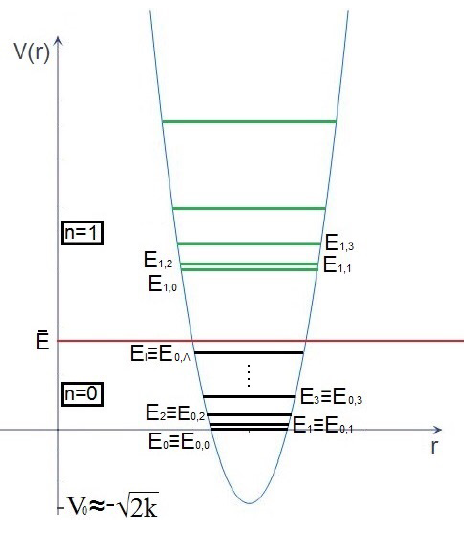
\includegraphics[width = \textwidth/2]{images/FioreEigenvalues.PNG}
    \caption{Eigenvalues of the Hamiltonian for steep enough potential for $D = 2$. The cutoff energy $\cut E$ can be chosen so that the energies below it are the spectrum of the free Hamiltonian $L^2$ in $S^d$.}
    \label{fig:D2EigenvaluesEigenEnergiesHarmonicCutoff}
\end{figure}

As illustrated in \ref{fig:D2EigenvaluesEigenEnergiesHarmonicCutoff}, we will see that, if $\cut E$ is chosen small enough with respect to $k$, e.g. $\cut E \lesssim 8\sqrt{k}$, the eigenvalues of $H$ below $E_{1,0}$ will be a truncation of the spectrum of $L^2$, i.e. the smallest eigenvalues of $H$ will be (approximately) $j(j+D-1)$ for $j = 1, 2, \dots, \Lambda$ for some positive integer $\Lambda$. This introduces the second main ingredient of our construction: \textit{the energy cutoff}. In general, \rtext{for any given $D = d + 1 \in \ZZ_{\geq 2}$, first suppose that $k$ is sufficiently steep to make the eigenvalue $E_{1, 0}$ be above the cutoff energy $\cut E$, %\dbtext{but also that $\cut E$ is high enough so that no eigenvalues are between it and $E_{1, 0}$} 
then, we will define the algebra \lbtext{$\acal_{\cut E}$} as the algebra of operators over the finite dimensional Hilbert space \lbtext{$\hcal_{\cut E}$}, spanned by the solutions $\psi_{0, j} \equiv \psi_j$ of the Schrodinger equation (under the harmonic approximation \ref{harmonicApproximationRadialSolutionGeneralD}) whose energies $E_{0, j} \equiv E_j$ are below $\cut E$}.

In order to make a fuzzy space $\{\acal_\Lambda\}_{\Lambda \in \NN}$ out of this construction of algebras $\acal_{\cut E}$, we need to make $\cut E$ and $k$ grow with a $\Lambda \in \NN$ in such a way that: 1. $k$ is big enough to not produce radial excitations, i.e. keep nontrivial radial eigenfunctions, for which the label $n \geq 1$, above the cutoff; 2. for fixed $\Lambda$, the extremum eigenvalues are $\Lambda(\Lambda + D - 2)$. This may be done, for example, by choosing 
\begin{align}
    \cut E = \cut E(\Lambda) &= \Lambda(\Lambda + d - 1) & k = k(\Lambda) \geq \Lambda^2(\Lambda + 1)^2.
\end{align}

%%%%%%%%%%%%%%%%%%%%%%%%%%%%%%%%%%%%%%%%%%%%%%%%%%%%%%%%%%%%%%%%
%%%%%%%%%%%%%%%%%%%%%%%%%%%%%%%%%%%%%%%%%%%%%%%%%%%%%%%%%%%%%%%%
\section{Construction of $\acal_{\cut E}$ for $D = 2$}

{
    \color{gray}
    
    - Equation \eqref{eqn9} has the approximation, where $\rho := \ln r$
    \begin{equation}
        \label{harmonic2D}
        \hat H f(\rho) = e_m f(\rho), \qquad
        \hat H = - \partial_\rho^2 + k_m(\rho - \tilde \rho_m)^2,
    \end{equation} $
        k_m := 2(k - E'), \quad
        E' := E - V_0, \quad
        \tilde \rho_m := \frac{E'}{k_m}, \quad
        e_m = \frac{E'^2}{k_m} + E' - m^2
    $
    - The solutions $f_{n,m}$ are known, $n \in \bb N, m \in \ZZ$ \then $e_{m, n}(k) = (2n+1)\sqrt{k_m}$ \then $E'_{m,n}(k)$ satisfies a quartic equation \then $E_{m,n}(k, V_0)$.
    
    - Fixing $V_0 = V_0(k)$ such that $E_{0, 0} = 0$ \then $V_0(k) = -\sqrt{2k} + 2 - \frac{7}{2}\frac{1}{\sqrt{2k}} + o(1/k)$ and 
    $\sum_{n = -1}^\infty v_n \left( \sqrt{\frac{1}{k}} \right)^n \approx -\sqrt{2k} + 2 - o(1/k)$ \then
    \begin{equation}
        \rtext{E_{n, m}(k)} = m^2 + 2n\sqrt{2k} - 2n + o(1/\sqrt{k})
    \end{equation}
    
    - Choosing $\cut E < 2 \sqrt{2k} - 2$, the spectrum of $H$ is a truncation of $L^2$: \textbf{the radial oscillations are ``frozen''}: $\cut{\partial_r} = 0$.
    \begin{multline*}
        \lbtext{\psi_m(\rho, \phi)} := f_{0, m}(\rho) e^{im\phi} = c_m e^{im\phi}exp{\left[ -\frac{(\rho - \tilde \rho_m)^2 \sqrt{k_m}}{2} \right]} \\\xrightarrow{k \to \infty} \delta(r-1)e^{i m \phi}
    \end{multline*}
    \begin{equation}
        E = E_m(k) = m^2 + o(1/\sqrt{k})
    \end{equation}
    
    - For $\lbtext{\Lambda} := \lfloor \cut E \rfloor$, 
    \begin{align}
        \lbtext{\hcal_{\Lambda}}:= \lbtext{\hcal_{\cut E}} := span\{\psi_m\}_{|m| \leq 
    \lfloor \cut E \rfloor} ,
    \lbtext{\acal_\Lambda} := \mathcal B(\hcal_\Lambda)
    \end{align}
    
    - Since $H$ generates the time evolution, a
    An element of $\hcal_\Lambda$ doesn't evolve out of $\hcal_\Lambda$.
    
    - Get a fuzzy space: e.g. choosing $k = \Lambda^2(\Lambda+1)^2$ --make $k$ diverge with $\Lambda$ while $\nu_{\cut E}$ goes to $\{r = 1\}$
    
    - This cutoff entails replacing every observable by $A \mapsto \lbtext{\cut A} = P_{\cut E} A P_{\cut E}$% \dbtext{when?}
}

\linea

When decomposing the eigenfunctions of the Schrodinger equation into radial and angular components, $\psi(r, \phi) = \tilde f(r) Y(\phi)$, the angular equation $L^2 Y = EY$ for $D = d+1 = 2$ is 
\begin{equation}
    - \partial_\phi^2 Y = E Y
\end{equation}
since the only angular momentum component is $L_{12} = - L_{21} =: L = -i(x^1 \partial_2  - x_2 \partial_1) = - i \partial_\phi$. The \dbtext{spherical harmonics} are, then, labeled by an integer $m$ and:
\begin{align}
    Y_m(\phi) &= e^{im \phi} & m \in \ZZ\\
    E_m &= m^2.
\end{align}

\lin

Defining $\rho := \ln r$ and $f(\rho) := \tilde f(r)$, the radial equation \ref{equationRadialSchrodingerGeneralDPolarAngles} becomes $f''(\rho) + \{e^{2\rho} [E - V(e^\rho)] - m^2 \} f(\rho) = 0$, and expanding $e^{2\rho}$ about $\rho = 0$ we obtain the following harmonic approximation of the radial equation \ref{equationRadialSchrodingerGeneralDPolarAngles}: 
\begin{equation}\label{equationHarmonicApproximation2DRadial}
        [- \partial_\rho^2 + k_m(\rho - \tilde \rho_m)^2] f(\rho) = e_m f(\rho),\text{ where}
\end{equation}
\begin{equation}\label{equationConstantsHarmonicApproximationRadialD2}
        k_m := 2(k - E'_m),\quad 
        E'_m := E_m - V_0,\quad 
        \tilde \rho_m := \frac{E'_m}{k_m},\quad
        e_m = \frac{E'^2_m}{k_m} + E'_m - m^2.
\end{equation} 
When solving this equation, taking into account that $\psi = f(\rho) $ an additional label $n \in \ZZ_{\geq 0}$ appears to label the eigenvalues of the previous equation; these solutions are:
\begin{eqnsplit}
    f_{n, m}(\rho) &= \exp\{\left[ - \frac{(\rho - \tilde \rho_m \sqrt{k_m})}{2}\right]\} H_n\left[ (\rho - \rho_m)\right]\\
    e_{n, m} &= (2n+1) \sqrt{k_m},
\end{eqnsplit}
where $H_n$ are the Hermite polynomials, $H_n$ being a polynomial of degree $n$ on the dependent variable; in particular, $H_0 = 1$.

From equation \ref{equationConstantsHarmonicApproximationRadialD2} it follows that $E'_m \equiv E'_{n, m} = E_{n, m} - V_0$ satisfies
\begin{equation}\label{equationAlmostQuarticDeterminesE'}
    \frac{E'_{n, m}}{2(k - E'_{n, m})} + E'_{n, m} - m^2 = (2n+1) \sqrt{2(k - E'_{n, m})};
\end{equation}
by squaring both sides we obtain a quartic equation for $E'_{n,m}$ that makes it a function of $k$, and hence we obtain the original eigenvalues of the approximate Schr\"odinger equation $E_{n,m}$ as a functions of $k$ and $V_0$.

\lin

As was mentioned in the previous section, in order to get simple eigenenergies we fix $V_0$ such that the ground energy $E_{0, 0}$ equals $0$. To do this we replace use the tags $m = n = 0$ in equation \ref{equationAlmostQuarticDeterminesE'} and use $E_{0, 0} = 0$. From there, we deduce that $V_0$ has a quartic equation that determines it a function of $k$, which can be rewritten as
\begin{equation}\label{equationV0AlternativeNotQuartic}
    - \sqrt{\frac{1}{2k}}V_0 - \left( \sqrt{\frac{1}{2k}} \right)^3 V_0^2 = \left( 1 + \frac{V_0}{k} \right)^\frac{3}{2}
\end{equation}
. Although a closed formula of $V_0(k)$ is possible, we opt for finding its Taylor expansion with respect to the variable $1/\sqrt{k}$ by using the implicit formula for $V_0(k)$; the resulting formula is:
\begin{equation}\label{equationFormulaExpansionV0functionOfK}
    V_0(k) = - \sqrt{2k} + 2 - \frac{7}{2} \frac{1}{\sqrt{2k}} + o\left(\frac{1}{k}\right).
\end{equation}\todo{check that $o$}
Finally, this expansion in $k$ of $V_0$ induces the following expansion of the eigenenergies of the harmonic approximation of Schrodinger equation:
\begin{equation}\label{equationEigenEnergies2DSchrodingerSolutionsHarmonicApproximation}
    E_{n, m} = m^2 + 2n\sqrt{2k} - 2n + o\left(\frac{1}{\sqrt{k}}\right).
\end{equation}

\lin 

The final step to build the Hilbert space $\hcal_{\cut E}$ and $\acal_{\cut E}$ given a cutoff energy $\cut E \geq 0$, is to make sure that $k$ is steep enough to ensure that $E_{1, 0}$ is above it, and for this is expressed by the inequality
\begin{align}
    \cut E < E_{1, 0} \approx 2 \sqrt{2k} - 2.
\end{align}\todo{perhaps the $o(1/\sqrt{k})$ term is negative?}
In that case, renaming $\psi_{0, m}$ and $E_{0, m}$ as $\psi_m$ and $E_m$ for $m \in \ZZ$, we define the spaces
\begin{eqnsplit} \label{equationDefinitionOFHandEHilbertAndAlgebraGivenCutoff}
    \hcal_{\cut E} &:= span\{ \psi_m(\rho, \phi) \,:\, E_m \leq \cut E \}\\
    \acal_{\cut E} &:= End(\hcal_{\cut E});
\end{eqnsplit} where
\begin{equation}\label{equationDefinitionPsimD2BasisOfHCutE}
    \psi_m(\rho, \phi) = c_m e^{im\phi} \exp \left[ - \frac{(\rho - \tilde \rho_m) \sqrt{k_m}}{2} \right], \quad \text{where}
\end{equation}
\begin{align}\label{equationExpansionKDependentConstantsPsim}
    k_m &= 2k \left( 1 - \frac{2}{\sqrt{2k}} + \frac{2-m^2}{k} + o\left( \frac{1}{k^{3/2}} \right) \right), &
    \tilde \rho_m &= \frac{1}{\sqrt{2k}} + \frac{m^2}{2k} + o\left( \frac{1}{k^{3/2}} \right).
\end{align}

Notice that, in principle, the definition of $\acal_{\cut E}$ is dependent on the chosen $k$ due to $k_m$ and $\tilde \rho_m$, so we may write instead $\psi_{n, m}(\rho, \phi)$ as $\psi_{n, m}(\rho, \phi; k)$; also notice that, for a fixed $k$ and two cutoffs $\cut E_1$ and $\cut E_2 > \cut E_1$ compatible with this $k$, then $\hcal_{\cut E_1}$ is, strictly, a subspace of $\hcal_{\cut E_2}$ since its basis elements $\psi_m$ are also basis elements of the latter, but only due to the fixed choice of $k$ for both cutoffs. 
However, first notice since $k$ is chosen large, all $\psi_m$ essentially vanish outside the $k$ dependent region $\nu_{\cut E}$, for $m$ fixed, and in fact $\psi_m(\rho, \phi) \to e^{im\phi} \delta(\rho - 1)$ in probability as $k \to \infty$; more importantly, the dependence on $k$ of the definition of $\acal_{\cut E}$ will not be relevant to our studies, since all what we will need in order to study the fuzzy spaces they form are the fact that they are endomorphism algebras over finite dimensional Hilbert spaces, and their behavior under the action of the group $O(2)$ induced by the action on the underlying Hilbert space. In fact, it is easy to see (since $O(2)$ doesn't affect the radial coordinate) that, for any compatible $k$, $\hcal_{\cut E}$ is isomorphic to  $\hcal'_{\cut E} := span\{e^{i m \phi} \, : \, m \in \ZZ, \, m^2 \leq \cut E\}$ in an $O(2)$-equivariant way, and, hence, that \rtext{$\acal_{\cut E}$\todo{again, strictly speaking, I am assuming that the extra factor in the $k$-expansion of the energies is positive} is isomorphic to $\acal'_{\cut E} := End(\hcal'_{\cut E})$ as a $C^*$-algebra and as a representation space of $O(2)$}.


Now, to parametrize these algebras by $\Lambda \in \NN$, define
\begin{eqnsplit}
    \hcal_\lambda &:= \hcal_{\Lambda = \lfloor \cut E \rfloor} \\
    \acal_\Lambda &:= End(\hcal_\Lambda);
\end{eqnsplit}
this means that the energies of the basis elements of $\hcal_\Lambda$ are all those $m^2$ that are below the energies $E_{1,0}$. Strictly speaking, to define each $\acal_\Lambda$ we also need to choose $k$ as a function on $\Lambda$ in such a way that it diverges with $\Lambda$ and that $k(N)$ is compatible with the cutoff energy $\Lambda$, for this,  equation \eqref{ } tells us that we can choose any function
\begin{equation}
    k(\Lambda) \geq \Lambda^2 (\Lambda + 1^2).
\end{equation}


%%%%%%%%%%%%%%%%%%%%%%%%%%%%%%%%%%%%%%%%%%%%%%%%%%%%%%%%%%%%%%%%
%%%%%%%%%%%%%%%%%%%%%%%%%%%%%%%%%%%%%%%%%%%%%%%%%%%%%%%%%%%%%%%%
\section{Important Observables and their Commutation Relations}

{
    \color{gray}
    
    - Up to infinite, $1/k^{1/2}\dbtext{?}$ and $1/k^{3/2}$ orders, respectively
    \begin{align}
    \label{projObs2D}
        \rtext{\cut L} \psi_m &= m \psi_m; & 
        \rtext{\cut H} &= \cut L^2; & 
        \rtext{\cut x^\pm} \psi_m = 
            \begin{cases}
                \frac{a}{\sqrt{2}} \sqrt{ 1 + \frac{m(m \pm 1)}{k} } \psi_{m \pm 1} & -\Lambda \leq \pm m \leq \Lambda - 1 \\
                0 & \text{otherwise}
            \end{cases}
    \end{align}
    - And so, up to terms of $1/k^{3/2}$
    \begin{align}
        \label{conmObs2D}
        \cut{x^+}^\dagger &= \cut{x^-}; &
        [\cut L, \cut{x^\pm}] &= \pm \cut{x^\pm}; &
        \rtext{[\cut{x^+}, \cut{x^-}]} &= - \frac{\cut L}{k} + \left[1 + \frac{\Lambda(\Lambda+1)}{k}\right] (\tilde P_{\Lambda} - P_{-\Lambda})a^2.
    \end{align}
     - If \eqref{projObs2D} are used exactly to define elements of $\mathcal B(\hcal_\Lambda) \equiv \acal_\Lambda$ then \eqref{conmObs2D} are also exact, and $\cut{x^\pm}$ generate $\acal_\Lambda$. -- $\cut{\partial_\pm}$ are now redundant... but I'm not sure why
     
}

\linea


%%%%%%%%%%%%%%%%%%%%%%%%%%%%%%%%%%%%%%%%%%%%%%%%%%%%%%%%%%%%%%%%
%%%%%%%%%%%%%%%%%%%%%%%%%%%%%%%%%%%%%%%%%%%%%%%%%%%%%%%%%%%%%%%%
\section{Realization of $\acal_\Lambda$ through $U\soth$}

{
    \color{gray}
    
    - $O(2)$ acts on $\hcal_\Lambda \subset L^2(\RR^2)$, and so \rtext{on $\acal_\Lambda$}, since $[H, O(2)\cdot ] = 0$. through the action induced in $\acal_\Lambda$ by its action on $\RR^2$.
        \begin{itemize}
            
        \item \textit{Rotation} $R_\theta$: $\cut{x^\pm} \mapsto e^{\pm i \theta} \cut{x ^\pm}; \cut L \mapsto \cut L \in \acal_\Lambda$.
        
        \item \textit{Reflection}: $\cut{x^\pm} \mapsto -\cut{x^\mp}; \cut L \mapsto -\cut L$.
        
        \end{itemize}
    
    - \rtext{We can consider \otext{$\acal_\Lambda \cong  M_N(\CC) = \pi_\Lambda(Uso(3))$} \textbf{as a $*$-algebra and representations of $O(2)$}}, where $\pi_\Lambda$ is the $\lbtext{N} := 2 \Lambda + 1$ dimensional representation. $SU(N) \ni g$ is the group of $*$-automorphisms of $M_N(\CC) \cong \acal_\Lambda$ acting by $a \mapsto g a g^{-1}$; $O(2)$ is then a subgroup. Comes from mapping:
    \begin{align}
        \rtext{\cut{x^\pm}} &\longleftrightarrow \rtext{f_\pm (J^0) J^\pm}, &
        \rtext{\cut L }& \rtext{\longleftrightarrow J^0}
    \end{align}
    where $J^\pm, J^0$ is the Weyl-Cartan basis of $so(3)$, $\lbtext{f_\pm(s)} := \frac{1}{\sqrt{2}} \sqrt{\frac{1 + s(s-1)/k}{\Lambda (\Lambda + 1) - s(s-1)}} =: \lbtext{f_-(-s)}$%: $[J^+, J^-] = J^0; [J^\pm, J^0] = \pm J^\pm$

    - $O(2) \subset SO(3)$: \textit{Rotation}: $\pi_\Lambda(e^{i \theta J_0})$; \textit{Refl.}: $\pi_\Lambda(e^{i\pi (J^+ + J^-)/\sqrt{2}})$
    
    \lin 
    
    Let $(V_l, \pi_l)$ be the irreducible representations of $O(3)$ characterized by $L^2 = l(+1)$
    
        \begin{itemize}
        
        \item  \begin{equation}
            \hcal_\Lambda \cong \bigoplus_{l = 0}^\Lambda V_l
        \end{equation}
        
        \item \begin{equation}
            C_\Lambda \cong \bigoplus_{l = 0}^{2\Lambda} V_l
        \end{equation}
        
        \end{itemize}
        
    \rtext{\textbf{As $\Lambda \to \infty$ these respectively become the decomposition of $L^2(S^2)$ \& of $C(S^2)$ that acts on $L^2(S^2)$.}}
}

\linea


%%%%%%%%%%%%%%%%%%%%%%%%%%%%%%%%%%%%%%%%%%%%%%%%%%%%%%%%%%%%%%%%
%%%%%%%%%%%%%%%%%%%%%%%%%%%%%%%%%%%%%%%%%%%%%%%%%%%%%%%%%%%%%%%%
\section{Convergence}

{
    \color{gray}
    
    - \textbf{$\psi_m$ as fuzzy analogues of $e^{i m \phi} \in \hcal$}: $O(2)$-covariant embedding $\hcal_\Lambda \hookrightarrow \otext{\hcal = L^2(S^1)}$, $\psi_m \mapsto e^{im\phi}$; \hfill \\then $\hcal_\Lambda \to \hcal$ as $\Lambda \to \infty$ in the sense that $\forall \phi \in \hcal$, $\lbtext{\phi_\Lambda} := \sum_{|m| \leq \Lambda} \phi_m e^{im\phi} \to \phi$ in the $L^2$-norm.
    
    - Induces, \rtext{embedding $\acal_\Lambda \hookrightarrow \otext{\acal = \mathcal B(\hcal)}$ and limit $\acal_\Lambda \to \acal$} as $\Lambda \to \infty$.
    
    - \textbf{Fuzzy analogue of $B(S^1)$ of (bounded) functions on $S^1$} as subalgebra (act by mult.) of $\mathcal B(\hcal)$: $\lbtext{C_\Lambda} := \left\{ \sum_{h = -2\Lambda}^\Lambda f_h \eta^h \,|\, f_h \in \CC\right\}$ where $\eta^\pm  = \frac{\sqrt{2}}{a}x^\pm$ (so $\eta^\pm \to e^{\pm i \phi}$ as operators).
    
    - Choosing $k(\Lambda) \geq 2 \Lambda(\Lambda + 1)(w\Lambda+1)^2$, then \rtext{$B(S^1) \to \mathcal B(\hcal)$ as operators} due to the strong limits: $\hat f_\Lambda \to f\cdot$, $\hat{(fg)}_\Lambda \to fg\cdot $, $\hat f_\Lambda \hat g_\Lambda \to fg\cdot$, where $\lbtext{\hat f_\Lambda} := \sum_{h = -2\Lambda}^{2\Lambda} f_h \eta^h$ is ``truncation'' of $f \in B(S^1)$.
    
}

\linea



%%%%%%%%%%%%%%%%%%%%%%%%%%%%%%%%%%%%%%%%%%%%%%%%%%%%%%%%%%%%%%%%%%%%%%%%%%%%%%
%%%%%%%%%%%%%%%%%%%%%%%%%%%%%%%%%%%%%%%%%%%%%%%%%%%%%%%%%%%%%%%%%%%%%%%%%%%%%%
%%%%%%%%%%%%%%%%%%%%%%%%%%%%%%%%%%%%%%%%%%%%%%%%%%%%%%%%%%%%%%%%%%%%%%%%%%%%%%
\chapter{Systems of Coherent States on the New Fuzzy Spheres}\label{chp:CHNew}

% { \color{gray}

% \lin


% \cite{FioreTheCase2020}
% -- Coherent states are, apparently, crucial if we want these spaces to have applications

% -- The weak system of coherent states $\mathcal W^d$ is made of the states minimizing $(\Delta \vec x)^2$: they are related to the diagonalization of the coordinates $x_i$; they are $O(D)$-invariant.

% -- A class of $O(D)$-invariant strong SCS are introduced, and in particular an interesting one is $\mathcal S^d$ which minimizes, within this class of CS, $(\Delta \vec x)^2$

% -- The diagonalization of the position observables seems to be improved on their last paper

% \lin

% }


As previously mentioned in the introduction, coherent states of an algebraic space associated to a Hilbert space \todo{Asegurarme de hablar de la importancia de estados coherentes en la introduccion!} are concrete objects with defined properties that enable the application of these spaces. In this chapter we describe some families of coherent states on the new fuzzy circle $S^1_\Lambda$, and study their localization properties for both position and angular momentum. 

Coherent states are vectors of the underlying Hilbert spaces, and so they induce states of the algebra. Our purpose will be to eventually study the distance between the family of states described in this document.

Throughout this chapter let $\hcal_\Lambda$ and $\acal_\Lambda$ be defined as in definition \ref{definitionHLambdaALambdaD2} for some $\Lambda \in \NN$ and some appropriate function $k = k(\Lambda)$ satisfying the inequality \eqref{inequationInequalityNeededforKasFunctionLambdaD2}, where $\{\psi_m\}_{|m| \leq \Lambda}$ given in \eqref{equationDefinitionPsimD2BasisOfHCutE} are an orthonormal basis of $\hcal_\Lambda$ composed of eigenvalues of $\cut L \in \acal_\Lambda$. Additionally, let the operators $\cut L$ and $\chi^\pm \in \acal_\Lambda$ be defined as in section \ref{chNewFuzzySectionObservables}, but let us use the symbol $L$ instead of $\cut L$. We will call $L$ the angular momentum observable and $\chi^1 = \frac{1}{2}(\chi^+ + \chi^-)$ and $\chi^2 = \frac{1}{2i}(\chi^+ - \chi^-)$ the position observables.

% \section{Localization}
% %%%%%%%%%%%%%%%%%%%%%%%%%%%%%%%%%%%%%%%%%%%%%%%%%%%%%%%%%
Given vector $\psi \in \hcal_\Lambda$, we will use the following measure of the localization of the vector in configuration space:
\begin{equation}
    (\Delta \vec x)^2 = \sum_{i = 1}^D (\Delta x^i)^2 = \langle (\vec x - \langle \vec x \rangle)^2 \rangle = \langle \vec x^2 \rangle - \langle \vec x \rangle ^2,
\end{equation}
where the expectation value for any observable $A$ is
\begin{equation}
    \langle A \rangle = \langle \psi | A | \psi \rangle.
\end{equation}

Similarly, for localization on momentum space the measure will be:
\begin{equation}
    (\Delta \cut L)^2 = \langle (\cut L - \langle L \rangle )^2 \rangle = \langle L^2 \rangle - \langle L \rangle ^2;
\end{equation}
from now on we will denote $\cut L \in \acal_{\Lambda}$ simply by $L$.

\section{Angular Momentum Saturating Coherent States}
%%%%%%%%%%%%%%%%%%%%%%%%%%%%%%%%%%%%%%%%%%%%%%%%%%%%%%%%%

The orthonormal basis $\{\psi_m\}_{|m| \leq \Lambda}$ is our first family of coherent states. 

The group 
\begin{equation}
    G = \{S^n e^{i(aL + b)} \,:\, (a, b, n) \in \RR^2 \times \ZZ_{2\Lambda + 1}\} \cong U(1) \times U(1) \rtimes \ZZ_{2\Lambda + 1}
\end{equation}
where $S$ is the ladder operator defined in \ref{definitionLadderOperatorsHLambda}, with operation
\begin{equation*}
    S^n e^{i(aL+b)}\, S^{n'}e^{i(a'L+b')} = S^{n + n'} e^{i[(a+a')L + (b + b' + an')]},
\end{equation*}
acts unitarily, transitively and irreducibly on $\{\psi_m\}_{|m|\Lambda}$, and the isotropy subgroup $H$ of all $\psi_m$ under this group action is clearly
\begin{equation}
    H = \{e^{i(aL+b)} \,:\, (a, b) \in \RR^2 \} \cong [U(1)]^2.
\end{equation}
Hence 
\begin{equation}
    G/H = \{S^n \,:\, n \in \ZZ_{2\Lambda + 1}\} \cong \ZZ_{2\Lambda + 1},
\end{equation}
is the label space for the basis $\{\psi_m\}_{|m|\leq \Lambda}$. \todo{Do they maximize the isotropy subgroup? Is there an uncertainty relation, perhaps related to the Casimir (is this a Lie group? Semisimple?), that is minimized by this system of coherent states?}

Additionally, the fact that they are a basis means that we have the resolution of the identity
\begin{eqnsplit}\label{resolutionIdentityPsimHcalLambda}
    1_{\hcal_\Lambda} &= \sum_{ m = -\Lambda}^\Lambda \tilde P_m \\
    &= \int_{G/H} \tilde P_m \, d\mu(m),
\end{eqnsplit}
where $\mu$ is the counting measure on $G/H$, induced by the Haar measure on the Lie group $G$. Hence $\{\psi_m\}_{|m| \leq \Lambda}$ is a strong system of coherent states \ref{definitionSystemCoherentStates}.

Now, let's study the localization of these vectors. Since each $\psi_m$ is an eigenvalue of $L$, $(L - \langle L\rangle ) \psi_m = 0$, 
\begin{equation}
    (\Delta L)^2 = 0.
\end{equation}
Similarly, $\langle \psi_m | \chi^i | \psi_m \rangle = 0$, so. $\langle \chi^i \rangle = 0$ for each $i = 1, 2$, and therefore $(\Delta \chi^i)^2 = \langle (\chi^i)^2 \rangle$, and so
\begin{align}
    (\Delta \chi^i)^2 &= \begin{cases} \frac{1}{2} \left( 1 + \frac{m^2}{k} \right) & \text{if } |m| \leq \Lambda\\
    \frac{1}{4} \left[ 1 + \frac{\Lambda(\Lambda - 1)}{k} \right] & |m| \leq \Lambda \end{cases} &
    (\Delta \vec \chi)^2 &= \begin{cases} \left( 1 + \frac{m^2}{k} \right) & \text{if } |m| \leq \Lambda\\
    \frac{1}{2} \left[ 1 + \frac{\Lambda(\Lambda - 1)}{k} \right] & |m| \leq \Lambda \end{cases},
\end{align}
up to fourth order in powers of $1 / \sqrt{k}$.

This system of coherent states can be characterized by a system of uncertainty relations: the commutation relations \eqref{equationOperatorFormulaCommutatorsChiD2} have as consequence the following uncertainty relations:
\begin{align}\label{equationUncertaintyRelationsMomentumSpaceCharacterizeBasisPsimD2}
    (\Delta L)^2 (\Delta \chi^i)^2 &\geq \frac{1}{4}\langle \chi^i \rangle ^2,& (\Delta L)^2 (\Delta \vec \chi)^2 &\geq \frac{1}{4} \langle \vec \chi \rangle ^2.
\end{align}
The fact that $\langle \chi^i \rangle = (\Delta L)^2 = 0$ means that the system $\{\psi_m\}$ saturates these inequalities. In fact, more is true, as proven in \cite{FioreCoherent2020}:

\begin{proposition}
The basis $\{\psi_m\}_{|m|\leq \Lambda}$ is a system of coherent states that minimize the uncertainty relation \eqref{equationUncertaintyRelationsMomentumSpaceCharacterizeBasisPsimD2}.
\end{proposition}


%Family saturating $13_1$. IFF?\todo{}

\section{$SO(2)$-invariant Families of Strong Coherent States}
%%%%%%%%%%%%%%%%%%%%%%%%%%%%%%%%%%%%%%%%%%%%%%%%%%%%%%%%%

Let us now construct some families of strong coherent states by action of the compact group $SO(2)$ on each $\hcal_\Lambda$. Start with a unit vector $\omega = \sum_{m = -\Lambda}^\Lambda \omega_m \psi_m$. Acting on it with $e^{i \alpha L } \in  SO(2)$, for $\alpha \in [0, 2\pi)$
produces the unit vector
\begin{equation}
    \omega_\alpha := e^{i \alpha L} \omega = \sum_{m = -\Lambda}^\Lambda e^{im\alpha} \omega_m \psi_m,
\end{equation}
and associated to this vector define the orthogonal projection
$\tilde P_\alpha := | \omega_\alpha \rangle \langle \omega_\alpha|$. Define the operator $B \in \acal_{\Lambda}$ by $B := \int_0^{2\pi} d\alpha P_{\alpha}$, and notice that
\begin{equation*}
    B \psi_m = \int_{0}^{2\pi} d\alpha \, \omega_\alpha \overline{\omega_m} e^{-im\alpha} = \overline{\omega_m} \sum_{|n| \leq \Lambda} \omega_n \psi_n \int_0^{2\pi}d\alpha\, e^{i\alpha(n-m)} = 2 \pi |\omega_m|^2 \psi_m.
\end{equation*}
Hence, $B$ is proportional to the identity if and only if the norms $|\omega_m|$ are independent of $m$; since $\omega$ is unitary, this means that all $|\omega_m|^2$ have to be equal to $\frac{1}{2\Lambda + 1}$, and so
\begin{equation*}
    \omega_m = \frac{e^{i \beta_m}}{\sqrt{2\Lambda + 1}}
\end{equation*}
for some $\beta_m \in \RR/2\pi \ZZ$. 

In summary:

\begin{proposition}
All unit vectors $\omega$ for which their orbit under the action of $SO(3)$ generate a strong system of coherent states are parametrized by tuples $\beta \in (\RR/2\pi\ZZ)^{2\Lambda + 1}$:
\begin{equation}
    \omega^\beta := \sum_{m = -\Lambda}^\Lambda \frac{e^{i \beta_m}}{\sqrt{2\Lambda + 1}} \psi_m,
\end{equation}
and the resulting system of coherent states
\begin{align}
    \mathcal S^\beta_\alpha &:= \{\omega_\alpha^\beta\}_{\alpha \in [0, 2\pi)}, & 
    \omega^\beta_\alpha &= e^{i\alpha L} \omega^\beta = \sum_{m = -\Lambda}^\Lambda \frac{e^{i \beta_m + m \alpha}}{\sqrt{2\Lambda + 1}} \psi_m
\end{align}
induces the resolution of the identity
\begin{align}
    1_{\hcal_\Lambda} &= \frac{2\Lambda + 1}{2\pi} \int_0^{2\pi} d\alpha \, P^\beta_\alpha &
    P_\alpha^\beta := |\omega^\beta_\alpha \rangle\langle \omega^\beta_\alpha|.
\end{align}
\end{proposition}

For the strong system of coherent states $\{\omega^\beta_\alpha\}_{\alpha \in \RR/2\pi\ZZ}$ to further be $O(2)$-invariant, recall from  \eqref{equationTransformationO2OfeimphiHarmonicsCircled1} that the action of the inversion $F$ with respect to the $x^1$-axis transforms $\psi_m$ into $\psi_{-m}$, hence we may choose
\begin{align}\label{equationConditionBetasO2Invariant}
    \beta_{-m} &= \beta_m & \text{for all } m \in \ZZ_{2\Lambda + 1}
\end{align}
to get an $O(2)$-invariant system of coherent states.

With respect to the localization of the $SO(2)$-invariant coherent states first notice that $\langle L \rangle = 0$, and also that, since $x^+ = x^1 + i x^2$, $\langle x\rangle ^2 = |\langle x^+ \rangle|^2$, it can be shown that 
\begin{equation*}
    \langle x^+ \rangle = \frac{e^{-i\alpha}}{2\Lambda + 1} \sum_{m} e^{i( \beta_{m-1} - \beta_m)} \sqrt{1 + \frac{m(m-1)}{k}},
\end{equation*} 
up to second order in $1/\sqrt{k}$, and from this it is shown in \cite{FioreCoherent2020} that:
\begin{align}\label{equationLocalizationAllStrongSystemsCoherentD2}
    (\Delta L)^2 &= \langle L^2 \rangle = \frac{\Lambda(\Lambda + 1)}{3},&
    (\Delta \vec x)^2 = \frac{2 \Lambda}{2 \Lambda + 1} + \frac{2(\Lambda - 1)\Lambda (\Lambda + 1)}{3(2\Lambda + 1)k},
\end{align}
up to second order in $1/\sqrt{k}$. This means that $(\Delta \vec x)^2 = \langle x^2 \rangle - \langle x \rangle ^2$ is minimal when $\langle x \rangle ^2 = |\langle x^+ \rangle |^2$ is maximal, and this happens, by the triangle inequality, when $\beta$ is constant; in that case it is shown in \cite{FioreCoherent2020} that
\begin{equation}
    (\Delta \vec x)^2 < \frac{1}{\Lambda + 1} \left( \frac{1}{2} + \frac{1}{3\Lambda} \right) \overset{\Lambda \geq 2}{\leq } \frac{2}{3(\Lambda + 1)}.
\end{equation}
Notice that we might as well say that $\beta = 0$, since this represents a constant shift of phase for all elements of the system, and so \textit{the system of coherent states that minimize the spacial dispersion within the families of $SO(2)$-invariant strong systems is $O(2)$-invariant and is in a $O(2)$-equivariant correspondence with points in $S^1$ via the mapping $\omega^0_\alpha \leftrightarrow e^{i \alpha}$}.

Finally, notice that the unitary vectors $\omega^\beta_\alpha$ have no limit in $L^2(S^1)$ as $\Lambda \to \infty$ since their components with respect to the basis $\{\psi_m\}$ go to $0$; however, the vectors $\sqrt{2\Lambda + 1}\omega^0_\alpha$ have the limit $\delta_{\phi = \alpha}$ as a distribution, where these are vectors are multiples of the elements of a system of a $O(2)$-invariant system of coherent states that minimize, within this family, the spacial dispersion.

\section{Coherent States Minimizing the Square Distance}
%%%%%%%%%%%%%%%%%%%%%%%%%%%%%%%%%%%%%%%%%%%%%%%%%%%%%%%%%

Let $\mathcal{W}^1 \subset \hcal_\Lambda$ be theset of vectors that minimize the spacial dispersion $(\Delta \vec \chi)^2$. We can observe that since $\vec \chi^2$ and $\langle \vec x \rangle^2$ are $O(2)$-invariant, then $\mathcal W^1$ is invariant under $O(2)$ transformations. To give a more concrete description, first notice that equations \eqref{equationTransformationO2OfpsimhcalBasisD2} show that the spaces $W_m := \text{span}\{\psi_m\}$ for fixed $m \in \{-\Lambda, \dots, \Lambda\}$ are the irreducible subspaces of $\hcal_\Lambda$ under $SO(2)$, and that $\tilde W_{|m|} := \text{span}\{\psi_m, \psi_{-m}\}$ are the irreducible subspaces under the action of $O(2)$; \todo{Since the representation is not irreducible, I do not see why a single vector should generate all the set, i.e. there might be ``disconnected'' families within $W$}therefore, if we take a vector $\psi \in $ POR ALGUNA RAZON es u\todo{No lo veo, y es importante: ES Sistema de Estados Coherentes??}n sistema completo, es tambien un conjunto que puedo generar a partir de un vector, y ademas lo puedo generar a partir de solo $SO(2)$, y además lo puedo generar a partir de un vector $\xi$ tal que $\langle \chi^1 \rangle = 0$.

However, closed formulas for this coherent states might not be possible, in particular, because $\vec \chi^2 \neq 1$ unlike in quantum mechanics on a circle or on the fuzzy sphere. Instead, it is only true that $\vec \chi^2  = 1 + O(1/\Lambda^2)$ according to inequality \ref{inequationInequalityNeededforKasFunctionLambdaD2}; therefore, the minimization of $ (\Delta \vec \chi)^2 = \langle \vec \chi^2 \rangle - \langle \vec \chi \rangle ^2$ necessarily involves a simultaneous process of minimizing $\vec \chi^2 \rangle$ and maximizing $\langle \vec \chi\rangle ^2$. However, from the fact that $\vec \chi ^2 \psi_m  = (1 + O(1/\Lambda^2) )\psi_m$ (except for $m = \pm \Lambda$) and from the $O(2)$-equivariance of the spectrums of the position observables, it is \textit{expected \cite{FioreCoherent2020} that the eigenvectors $\tilde \psi$ of $\chi^1$ of highest eigenvalue, in absolute value, approximate $\psi$ at order $O(1/\Lambda^2)$}. However, from the graph \ref{fig:R2Chi} we observe that $\vec \chi^2$ is slightly greater the greater $m$ is and the smaller $\Lambda$ is, so this approximation might not work for very small $\Lambda$'s, but for $k(\Lambda) \geq \Lambda^2(\Lambda+1)^2$, although the difference between them is less than $2\%$ for $\Lambda \gtrsim 5$.

\begin{figure}
    \centering
    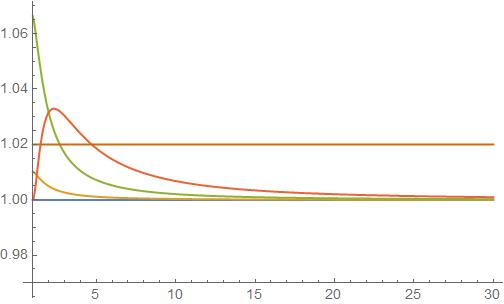
\includegraphics[width = \textwidth]{images/R^2.jpg}
    \caption{Square distance for various values of $m$ as a function of $\Lambda$, for $k(\Lambda) = \Lambda^2(\Lambda+1)^2$.}
    \label{fig:R2Chi}
\end{figure}

The operator $\chi^1$ has the following symmetric matrix representation
\begin{equation}
    X^\Lambda = \frac{1}{2} 
    \begin{pmatrix} 
    0 & b_\Lambda & 0 & 0& \cdots & 0& 0 & 0 \\
    b_\Lambda & 0 & b_{\Lambda - 1} & 0 & \cdots & 0 & 0 & 0\\
    0 & b_{\Lambda-1} & 0 & b_{\Lambda - 2} & \cdots & 0 & 0 &0\\
    \vdots & \vdots & \ddots & \ddots & \ddots & \vdots & \vdots & \vdots\\
    \vdots & \vdots & \vdots & \ddots & \ddots & \ddots & \vdots & \vdots\\
    \vdots & \vdots & \vdots & \vdots & \ddots & \ddots & \ddots & \vdots\\
    0 & 0 & 0 & 0 & \cdots & b_{2-\Lambda} & 0 & b_{1-\Lambda}\\
    0 & 0 & 0 &0 & \cdots & 0 & b_{1-\Lambda} & 0.
    \end{pmatrix}                                                                                                                           
\end{equation}
in the ordered basis $\{\psi_\Lambda, \psi_{\Lambda - 1}, \dots, \psi_{1-\Lambda}, \psi_{-\Lambda}\}$, where $b_m := \langle \psi_m | \chi^+ | \psi_{m-1} \rangle = \langle \psi_{m-1} | \chi ^- | \psi_m\rangle$ and so
\begin{equation}\label{equationbmD2}
    b_m = \begin{cases}
        \sqrt{1 + \frac{m(m-1)}{k}} + O\left( \frac{m^3}{k^{3/2}} \right), & \text{if } 1- \Lambda \leq m \leq \Lambda \\
        0, & \text{otherwise}.
    \end{cases}
\end{equation}

An additional approximation can be made by replacing the matrix $X^\Lambda$ by $X^\Lambda_0 = \lim_{\Lambda \to \infty} X^\Lambda$, which is the Toeplitz matrix where every nondiagonal entry of $X^\Lambda$ is replaced by a $1$; notice that the smallest value of $b_m$ is $1$ for $m = 0$ and it grows with the absolute value of $m$. Graph \ref{fig:bn} shows the value for the maximum $b_m$ as a function of $\Lambda$ assuming $k(\Lambda) = \Lambda^2(\Lambda+1)^2$. The eigenvectors and their corresponding eigenvalues of the operator $S^1 = \frac{S^+ + S^-}{2}$ represented by $X^\Lambda_0$ are:
\begin{align}
    \tilde \psi_{n} &= \sum_{m = -\Lambda}^\Lambda \sin{\left(\frac{(\Lambda + 1-m)(\Lambda + 1-n)\pi}{2\Lambda + 2}\right)} \psi_m,&
    \tilde \alpha_m &= \cos{\left(\frac{(\Lambda + 1-m)\pi}{2\Lambda + 2}\right)},
\end{align}
each vector with norm $\Lambda + 1$, and with $\tilde \alpha_{\Lambda} > \tilde \alpha_{\Lambda-1} > \cdots > \tilde \alpha_{-\Lambda} $.

\begin{figure}
    \centering
    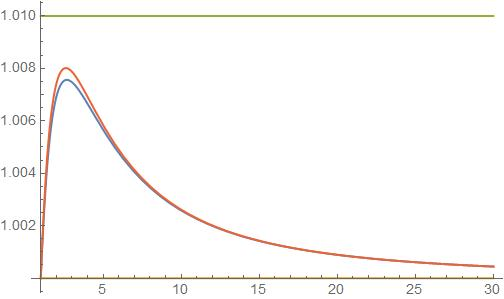
\includegraphics[width = \textwidth]{images/bn.jpg}
    \caption{Greatest $b_m$ as a function of $\Lambda$, for $k(\Lambda) = \Lambda^2(\Lambda+1)^2$. Red: $b_\Lambda$, Blue: approximation $b_\Lambda \approx \sqrt{1 + \frac{\Lambda(\Lambda - 1)}{k}}$. }
    \label{fig:bn}
\end{figure}

A good estimate, then, of the minimum dispersion is the dispersion of the eigenvector of $S^1$ with maximum absolute value eigenvalue $\tilde \alpha_{\pm \Lambda} = \cos{[\pi/(2\Lambda+2)]}$; in \cite{FioreCoherent2020} it is shown that for this vectors:
\begin{equation}
    (\Delta \vec \chi)^2 < \frac{3.5}{(\Lambda+1)^2} \overset{\Lambda \to \infty}{\longrightarrow} 0.
\end{equation}

The spectrum of $S^1$ satisfies that between any two subsequence eigenvalues in its spectrum for $\Lambda + 1$, $\Lambda_0^{\Lambda + 1}$, there is exactly one in $\Sigma_0^\Lambda$, and, furthermore, $\Sigma_0^\Lambda$ becomes uniformly dense in $[-1, 1]$ as $\Lambda \to \infty$. A similar result \cite{FioreXi2020, FioreTheCase2020} can be obtained for the spectrum of $\chi^1$:
\begin{theorem}
For all $\Lambda \in \NN$, denote the spectrum of $\chi^1$ for $\Lambda$ by $\Sigma^\Lambda_{\chi^1} = \{\alpha_k^\Lambda\}_{n = -\Lambda, \dots, \Lambda }$ ordered in increasing order with $n$. Then:
\begin{enumerate}
    \item If $\alpha$ belongs to $\Sigma^\Lambda_{\chi^1}$, then so does $-\alpha$.
    
    \item $\Sigma_{\Sigma_{\chi^1}}^\Lambda$ and $\Sigma_{\Sigma_{\chi^1}}^{\Lambda+1}$ interlace, i.e. between any two consecutive eigenvalues of $\chi^1$ for $\Lambda +1$, there is exactly one of $\chi^1$ for $\Lambda$:
    \begin{equation}
        \alpha_{\Lambda+1}^{\Lambda+1} > \alpha_{\Lambda}^{\Lambda} > \alpha_\Lambda^{\Lambda+1} > \alpha_{\Lambda-1}^{\Lambda} > \dots > \alpha_{-\Lambda}^{\Lambda} > \alpha_{-\Lambda-1}^{\Lambda+1}.
    \end{equation}
    
    \item $\Sigma_{\chi^1}^\Lambda$ becomes uniformly dense in $[-1, 1]$ as $\Lambda \to \infty$. In particular, $\alpha_{\Lambda}(\Lambda) \geq 1 - \frac{\pi^2}{8(\Lambda + 1)^2}$.
\end{enumerate}
\end{theorem}

In analogy with the study of distances in the fuzzy sphere, we expect this interlacing relation to be useful in the study of the relation between distances for contiguous $\Lambda$'s and for the study of the asymptotic behavior of the distance between this family of vectors.

%Recall that , then they also satisfy the criteria for position observables in $\acal_\Lambda$ given in section \ref{subsectionCriteriaGOodApproximationsOfPosition}, and in fact they also converge uniformly to the operators $e^{\pm i\phi}$ on $L^2(S^1)$ as specified in proposition \ref{theoremConvergesToQMD2}. Taking this definition, the special case in which $\Lambda = 1$ can be studied exactly \cite{FioreCoherent2020}. The eigenvectors of $\chi^1$ are:

%%%%%%%%%%%%%%%%%%%%%%%%%%%%%%%%%%%%%%%%%%%%%%%%%%%%%%%%%%%%%%%%%%%%%%%%%%%%%%
%%%%%%%%%%%%%%%%%%%%%%%%%%%%%%%%%%%%%%%%%%%%%%%%%%%%%%%%%%%%%%%%%%%%%%%%%%%%%%
%%%%%%%%%%%%%%%%%%%%%%%%%%%%%%%%%%%%%%%%%%%%%%%%%%%%%%%%%%%%%%%%%%%%%%%%%%%%%%
\chapter{Spectral Triples on the New Fuzzy Spheres}\label{chp:NewDistance}
\input{chapters/NewDistance}



%%%%%%%%%%%%%%%%%%%%%%%%%%%%%%%%%%%%%%%%%%%%%%%%%%%%%%%%%%%%%%%%%%%%%%%%%%%%%%
%%%%%%%%%%%%%%%%%%%%%%%%%%%%%%%%%%%%%%%%%%%%%%%%%%%%%%%%%%%%%%%%%%%%%%%%%%%%%%
\printbibliography

\end{document}
